%  Add 'draft' option to mark overfull boxes with black boxes
%  Add 'showkeys' option to make keywords appear
\documentclass[aps,prfluids,groupedaddress]{revtex4-2}
%\documentclass[aps,prl,preprint,groupedaddress]{revtex4-2}
%\documentclass[aps,prl,preprint,superscriptaddress]{revtex4-2}
%\documentclass[aps,prl,reprint,groupedaddress]{revtex4-2}

\usepackage{bm}
\usepackage{amsmath}
\usepackage{amssymb}
\usepackage{graphicx}
\usepackage{url}
\usepackage{xcolor}

% Mark up new/edited content in red for review.
\newcommand{\new}[1]{{\color{red}#1}}

%% OPTIONAL MACRO DEFINITIONS

% Dimensionless numbers
\newcommand{\Reyn}{\mathrm{Re}}

% math symbols
\newcommand{\rme}{\mathrm{e}}
\newcommand{\rmi}{\mathrm{i}}
\newcommand{\rmd}{\mathrm{d}}
\newcommand{\sym}{\mathrm{sym}}

% vectors small case
\newcommand{\bb}{\bm{b}}
\newcommand{\bc}{\bm{c}}
\newcommand{\be}{\bm{e}}
\newcommand{\bff}{\bm{f}}
\newcommand{\bg}{\bm{g}}
\newcommand{\bh}{\bm{h}}
\newcommand{\bmm}{\bm{m}}
\newcommand{\bn}{\bm{n}}
\newcommand{\bp}{\bm{p}}
\newcommand{\bq}{\bm{q}}
\newcommand{\br}{\bm{r}}
\newcommand{\bu}{\bm{u}}
\newcommand{\bv}{\bm{v}}
\newcommand{\bx}{\bm{x}}
\newcommand{\by}{\bm{y}}
\newcommand{\bz}{\bm{z}}

% vectors small case (greek letters)
\newcommand{\bchi}{\bm{\chi}}
\newcommand{\bmu}{\bm{\mu}}
\newcommand{\bomega}{\bm{\omega}}
\newcommand{\bphi}{\bm{\phi}}
\newcommand{\btau}{\bm{\tau}}
\newcommand{\btheta}{\bm{\theta}}

% vectors small case (latin)
\newcommand{\ba}{\bm{a}}

% vectors capital case
\newcommand{\bB}{\bm{B}}
\newcommand{\bC}{\bm{C}}
\newcommand{\bE}{\bm{E}}
\newcommand{\bF}{\bm{F}}
\newcommand{\bG}{\bm{G}}
\newcommand{\bH}{\bm{H}}
\newcommand{\bI}{\bm{I}}
\newcommand{\bK}{\bm{K}}
\newcommand{\bM}{\bm{M}}
\newcommand{\bN}{\bm{N}}
\newcommand{\bP}{\bm{P}}
\newcommand{\bQ}{\bm{Q}}
\newcommand{\bR}{\bm{R}}
\newcommand{\bS}{\bm{S}}
\newcommand{\bT}{\bm{T}}
\newcommand{\bU}{\bm{U}}
\newcommand{\bV}{\bm{V}}
\newcommand{\bW}{\bm{W}}
\newcommand{\bX}{\bm{X}}
\newcommand{\bTheta}{\bm{\Theta}}
\newcommand{\bOmega}{\bm{\Omega}}

% tensors
\newcommand{\tI}{\bm{\mathit{1}}}
\newcommand{\ta}{\bm{{a}}}
\newcommand{\tb}{\bm{{b}}}
\newcommand{\tc}{\bm{{c}}}
%
\newcommand{\tB}{\bm{{B}}}
\newcommand{\tC}{\bm{{C}}}
\newcommand{\tE}{\bm{{E}}}
\newcommand{\tEd}{\bm{\dot {E}}}
\newcommand{\tF}{\bm{{F}}}
\newcommand{\tG}{\bm{G}}
\newcommand{\tJ}{\bm{J}}
\newcommand{\tK}{\bm{{K}}}
\newcommand{\tM}{\bm{{M}}}
\newcommand{\tP}{\bm{{P}}}
\newcommand{\tPi}{\bm{{\Pi}}}
\newcommand{\tQ}{\bm{{Q}}}
\newcommand{\tR}{\bm{{R}}}
\newcommand{\tS}{\bm{{S}}}
\newcommand{\tT}{\bm{{T}}}
\newcommand{\tU}{\bm{U}}
\newcommand{\tsigma}{\bm{{\sigma}}}
\newcommand{\tepsilon}{\bm{{\epsilon}}}

% time derivatives of vectors
\newcommand{\bad}{\bm{\dot a}}
\newcommand{\bpd}{\bm{\dot p}}
\newcommand{\bqd}{\bm{\dot q}}
\newcommand{\brd}{\bm{\dot r}}
\newcommand{\bxd}{\bm{\dot \chi}}
\newcommand{\bthetad}{\bm{\dot \theta}}
\newcommand{\bEd}{\bm{{\dot E}}}
\newcommand{\bGd}{\bm{{\dot G}}}
\newcommand{\bQd}{\bm{{\dot Q}}}
\newcommand{\bRd}{\bm{{\dot R}}}
\newcommand{\bXd}{\bm{{\dot X}}}
\newcommand{\bThetad}{\bm{\dot \Theta}}

% unit vectors
\newcommand{\hz}{\bm{\hat z}}
\newcommand{\htheta}{\bm{\hat \theta}}
\newcommand{\hTheta}{\bm{\hat \Theta}}

% matrices
\newcommand{\mRot}{\bm{\mathcal{R}}}

% Math operators
\DeclareMathOperator{\cotan}{cotan}


\begin{document}

\title{Soft Mobility Theory}

\author{Christophe Eloy}
\affiliation{Aix-Marseille Univ, CNRS, Centrale Med, IRPHE, Marseille, France}
\email[]{celoy@centrale-med.fr}
%\homepage[]{Your web page}
%\thanks{}
\affiliation{Department of Applied Mathematics and Theoretical Physics, University of Cambridge, Cambridge, UK}

%\date{\today}

\begin{abstract}
Predicting how a deformable body moves and deforms in a viscous flow underlies problems ranging from microorganism locomotion to soft microrobotics, yet existing frameworks are either problem-specific or ill-suited to inverse design. We propose the soft mobility theory: applying the principle of virtual power and the Lorentz reciprocal theorem to a hyperelastic body in a background Stokes flow yields a configuration-dependent ordinary differential equation for the generalized coordinates of the body. This soft mobility equation extends classical rigid-body mobility theory in that the mobility, elastic, body-force, and flow-coupling tensors all depend explicitly on the instantaneous deformation. We specialize the framework to assemblies of hydrodynamically interacting spheres connected by elastic springs, using the Rotne--Prager--Yamakawa approximation to compute the mobility, and validate it on canonical problems spanning rigid and flexible bodies in quiescent and shear flows. An open-source JAX implementation makes entire simulations end-to-end differentiable. This allows efficient gradient-based inverse design: as proofs of concept, we recover the asymptotic optimum of a three-sphere swimmer and design a soft gyrotactic ``surfer'' that exploits passive deformation to ascend faster than its rigid counterpart in a Taylor–Green flow.
\end{abstract}

\maketitle

%%%%%%%%%%%%%%%%%%%%%%%%%%%%%%%%%%%%%%%%%%%%%%%%%%%%%%%%%%%%%%%%%%%%%%%%%%%%%
\section{Introduction\label{sec.intro}}

Microorganisms rely on their deformability to interact with the surrounding fluid \cite{Visser2001,Wheeler2019}. 
This deformation can be active when microswimmers propel themselves through their slender flagella and cilia~\cite{Lauga2009,Lauga2016,Lauga2020,Guasto2012,Wheeler2019}. It can also be passive, like red blood cells undergoing large shape changes as they flow through capillaries~\cite{BarthesBiesel2016,Farutin2013}, or diatoms using flexible structures such as mucilage stalks and fine spines to adapt their sinking velocity~\cite{Smayda1974,Wiseman1981,Padisak2003}. 
Across these systems, deformability is not incidental but functional, often conferring sensing, locomotion, or feeding advantages that a rigid body could not achieve.

In artificial systems, flexible fibers have been shown to buckle and tumble in quiescent, shear, and turbulent flows~\cite{Wiggins1998,Brouzet2014,Du-Roure2019,Zuk2021}, and a growing class of soft microrobots is being engineered for biomedical applications, such as in-situ sensing, drug delivery, and microsurgery~\cite{Sitti2021,Yasa2023,Tsang2020b,Elnaggar2024,Dabbagh2022,Mo2023,Jiang2022}.
Even microplastics deform and disperse in the ocean in ways that depend on their shape and flexibility~\cite{Sutherland2023}. 

These problems share a common physical structure: a deformable body whose shape evolves under the combined action of active, elastic, viscous, and body forces. 
This broad class of fluid--structure interactions is conventionally referred to as \emph{elastohydrodynamics}. 
We adopt here the more specific term \emph{soft mobility}, by which we mean the transport and deformation of a small deformable body immersed in a background flow, in direct analogy with the classical rigid-body mobility theory~\cite{Brenner1963,Happel2012,Kim2013}. 

Soft mobility encompasses both the \emph{forward} problem of predicting how a given soft body moves and deforms in a prescribed flow, and the \emph{inverse} problem of designing soft bodies to perform a target function: efficient locomotion, flow sensing, clustering, or autonomous navigation in complex environments. 
The latter is increasingly central to soft robotics~\cite{Kim2013a,Yasa2023} and embodied intelligence~\cite{Pfeifer2006}, and underlies the related notions of morphological computation~\cite{Pfeifer2014,Hauser2011,Hauser2014,Nakajima2015} and physical intelligence~\cite{Sitti2021,Hauser2023}, in which sensing, control, and decision-making are partly offloaded from a centralized processor to the mechanical response of the body itself.
Solving this inverse problem at low Reynolds number requires a specific approach, which we aim to develop in the present paper.

The natural starting point is the classical mobility theory developed in the 1960s for rigid bodies in Stokes flow~\cite{Brenner1963,Happel2012,Kim2013}. 
Owing to the linearity of the Stokes equations, the six-component velocity of a rigid body depends linearly on the applied force and torque and on the local background velocity, vorticity, and rate-of-strain. 
The mobility tensors entering this relation depend only on the body's shape and incorporate all the hydrodynamic complexity of the Stokes equations into a finite set of geometric coefficients. 
These tensors can be computed with different methods: boundary integral methods~\cite{Pozrikidis1992} that exploit Lorentz reciprocal theorem~\cite{Happel2012}, multiblob methods that discretize body surfaces with ``blobs''~\cite{Balboa-Usabiaga2017,Balboa-Usabiaga2022,Broms2023}, or slender-body theory for fibers~\cite{Tornberg2004,Nazockdast2017,Maxian2022}.
This formulation has recently been revived for complex-shaped macromolecules~\cite{Garcia-de-la-Torre1981,Zuk2014,Zuk2018} and reinterpreted as a low-dimensional dynamical system describing rigid-body sinking trajectories~\cite{Gonzalez2004,Witten2020}.
Its appeal, from the standpoint of the inverse problem, is the explicit, shape-dependent linear relation it provides between velocities and loads~\cite{Moreau2022}.

For $N$ rigid bodies, the same linear relationship extends to a $6N\times 6N$ grand mobility tensor encoding both single-body mobility and many-body hydrodynamic interactions. 
This tensor is at the core of Stokesian dynamics, which aims to simulate a large ensemble of rigid bodies interacting in a flow~\cite{Brady1988,Ichiki2002,Fiore2019,Swan2016}. 
To compute the grand mobility tensor efficiently, multipole expansions are generally used, such as the Rotne--Prager--Yamakawa (RPY) approximation, which provides a closed-form mobility for assemblies of spheres of possibly different radii~\cite{Rotne1969,Yamakawa1970,Wajnryb2013,Zuk2014,Cichocki2021}.
This approach is now mature for both passive rigid suspensions and active suspensions of rigid swimmers, routinely tackling problems with millions of degrees of freedom~\cite{Delmotte2015b}. 

A natural next step has been to leverage these tools to simulate deformable bodies by treating them as assemblies of rigid
sub-bodies linked by elastic or rigid constraints. 
For instance, bead models or multiblob methods approximate fibers as an ensemble of touching spheres connected by springs~\cite{Delmotte2015,Zuk2021,Fuchter2023}, and general articulated bodies can be simulated in a similar way~\cite{Balboa-Usabiaga2022}. 
At each timestep, however, these formulations require enforcing the constraints, which is a saddle-point linear system, typically solved via preconditioned iterative solvers (GMRES, FMM-accelerated iterations~\cite{Liang2013,Fiore2019}). 
This is efficient for forward simulation, but would be prohibitive for the inverse problem of shape optimization.

Closest in spirit to the present paper is the framework of Solovev and Friedrich~\cite{Solovev2021}. 
They explicitly project the deformation of a soft body onto a small set of generalized coordinates using Lagrangian mechanics.
This ``trick'' allows them to compute the dynamics of a shape-changing body without solving the constraints. 
In the conjugate space of generalized coordinates, they balance generalized hydrodynamic forces against active driving forces, which yields an explicit ordinary differential equation for the generalized velocities. 
Three differences with the present work should be noted. 
First, their framework is primarily designed for active microswimmers, not soft bodies deforming elastically. They model active bacterial flagella, eukaryotic cilia, and minimal model swimmers such as Purcell's three-link swimmer~\cite{Purcell2014} or Najafi's three-sphere swimmer~\cite{Najafi2004}.
Second, in their formulation, hydrodynamic forces are tabulated with boundary-element methods and interpolated, which makes it difficult to differentiate cleanly for gradient-based optimization. 
Third, their framework does not include the coupling to the background flow, which is essential for turbulent transport.

The goal of this paper is to develop a general ``soft mobility'' framework that simultaneously: 
(1) is derived from the continuum elastohydrodynamic problem of a hyperelastic body in a background Stokes flow; 
(2) accommodates arbitrary generalized coordinates and yields an explicit, configuration-dependent ordinary differential equation in which mobility, advection, and flow-gradient coupling tensors all appear; and 
(3) is constructed so that all tensors are smooth, differentiable functions of the design parameters, enabling end-to-end gradient-based inverse design.

The paper is organized as follows.
Section~\ref{sec.theory} formulates the continuum elastohydrodynamic
problem and derives its weak form via the principle of virtual power
and the Lorentz reciprocal theorem~\cite{Happel2012}. Section~\ref{sec.numerics}
specializes the framework to two finite-dimensional reductions --- a
Galerkin discretization on arbitrary basis modes and a
sphere-and-spring assembly --- and arrives at the soft mobility
equation in closed form, alongside the open-source Python
library~\cite{softmobility}. 
Section~\ref{sec.results} applies the framework to five canonical problems: gravity-driven sinking of a chiral rigid body and of a flexible fiber, the wrapping of a rotating clamped fiber, soft Jeffery orbits in shear, optimization of a three-sphere swimmer, and a soft gyrotactic surfer that exploits passive deformation to migrate through a Taylor--Green vortical flow. Section~\ref{sec.discussion} discusses extensions and applications.

%%%%%%%%%%%%%%%%%%%%%%%%%%%%%%%%%%%%%%%%%%%%%%%%%%%%%%%%%%%%%%%%%%%%%%%%%%%%%
\section{Problem formulation\label{sec.theory}}

%%%%%%%%%%%%%%%%%%%%%%%%%%%%%%%%%%%%%%
%\subsection{Hypotheses}

%%%%%%%%%%%%%%%%
%\subsubsection{Assumption of small Reynolds number}
We consider a deformable body of characteristic size $L$ immersed in a viscous fluid of kinematic viscosity $\nu$. 
The Reynolds number is $\Reyn = UL/\nu$, where $U$ is a characteristic velocity at the body scale. 
In turbulent environments, the Reynolds number can be calculated by using the Kolmogorov velocity $u_\eta=(\nu\varepsilon)^{1/4}$ as this characteristic velocity, such that $\Reyn = L/\eta$, with $\eta=(\nu^3/\varepsilon)^{1/4}$ the Kolmogorov length scale. An alternative choice is to estimate the characteristic velocity from the local velocity gradient. In that case, the characteristic velocity is $U \sim \|\nabla\bu^\infty\|L \sim L /\tau_\eta$, with $\tau_\eta = (\nu / \varepsilon)^{1/2}$ the Kolmogorov time scale, such that $\Reyn = (L/\eta)^2$. 

Throughout this work, we assume $\Reyn \ll 1$, so that inertia is negligible. 
Both choices yield $L\ll\eta$, where $\eta$ is the Kolmogorov length scale, as the condition for this approximation to hold. Under this assumption, the body is in quasi-static equilibrium at each instant, and the surrounding fluid obeys the Stokes equations.

%%%%%%%%%%%%%%%%
%\subsubsection{Background flow}
A further consequence of the small-Reynolds-number assumption is that the background flow $\bu^\infty(\br)$ can be linearized about a reference point $\br_0$ attached to the body,
\begin{equation}\label{eq:bg_flow}
\bu^\infty(\br) \approx \bu_0^\infty + \bomega_0^\infty \times (\br-\br_0)  + \tE_0^\infty \cdot (\br-\br_0),
\end{equation}
with $\bu_0^\infty$ the translational velocity, $\bomega_0^\infty = \frac{1}{2}\nabla\times\bu^\infty$ the angular velocity, and $\tE_0^\infty = \frac{1}{2}(\nabla\bu^\infty + \nabla^\top\bu^\infty)$ the rate-of-strain tensor of the background flow evaluated at $\br_0$.


%%%%%%%%%%%%%%%%%%%%%%%%%%%%%%%%%%%%%%
\subsection{Body}

%%%%%%%%%%%%%%%%
%\subsubsection{Hyperelastic material}
In its undeformed configuration, the body occupies a reference volume $\Omega_0$, with boundary $\partial\Omega_0$. % and an orthonormal body frame $(\be_1,\be_2,\be_3)$ is attached to it. 
Under the action of the flow and internal stresses, a material point $\bX\in\Omega_0$ is carried to its current position $\bx = \bchi(\bX,t)\in\Omega_t$ through the deformation map $\bchi$ (Fig.~\ref{fig:elastic_deformations}). The deformation gradient tensor $\tF = \partial\bchi/\partial\bX$ characterizes the local stretching and rotation of the material, and $J = \det\tF$ is its Jacobian. Mass conservation gives $\rho = \rho_0/J$, relating the density $\rho$ in the deformed configuration to its reference value $\rho_0$.

\begin{figure}[t]
\begin{center}
    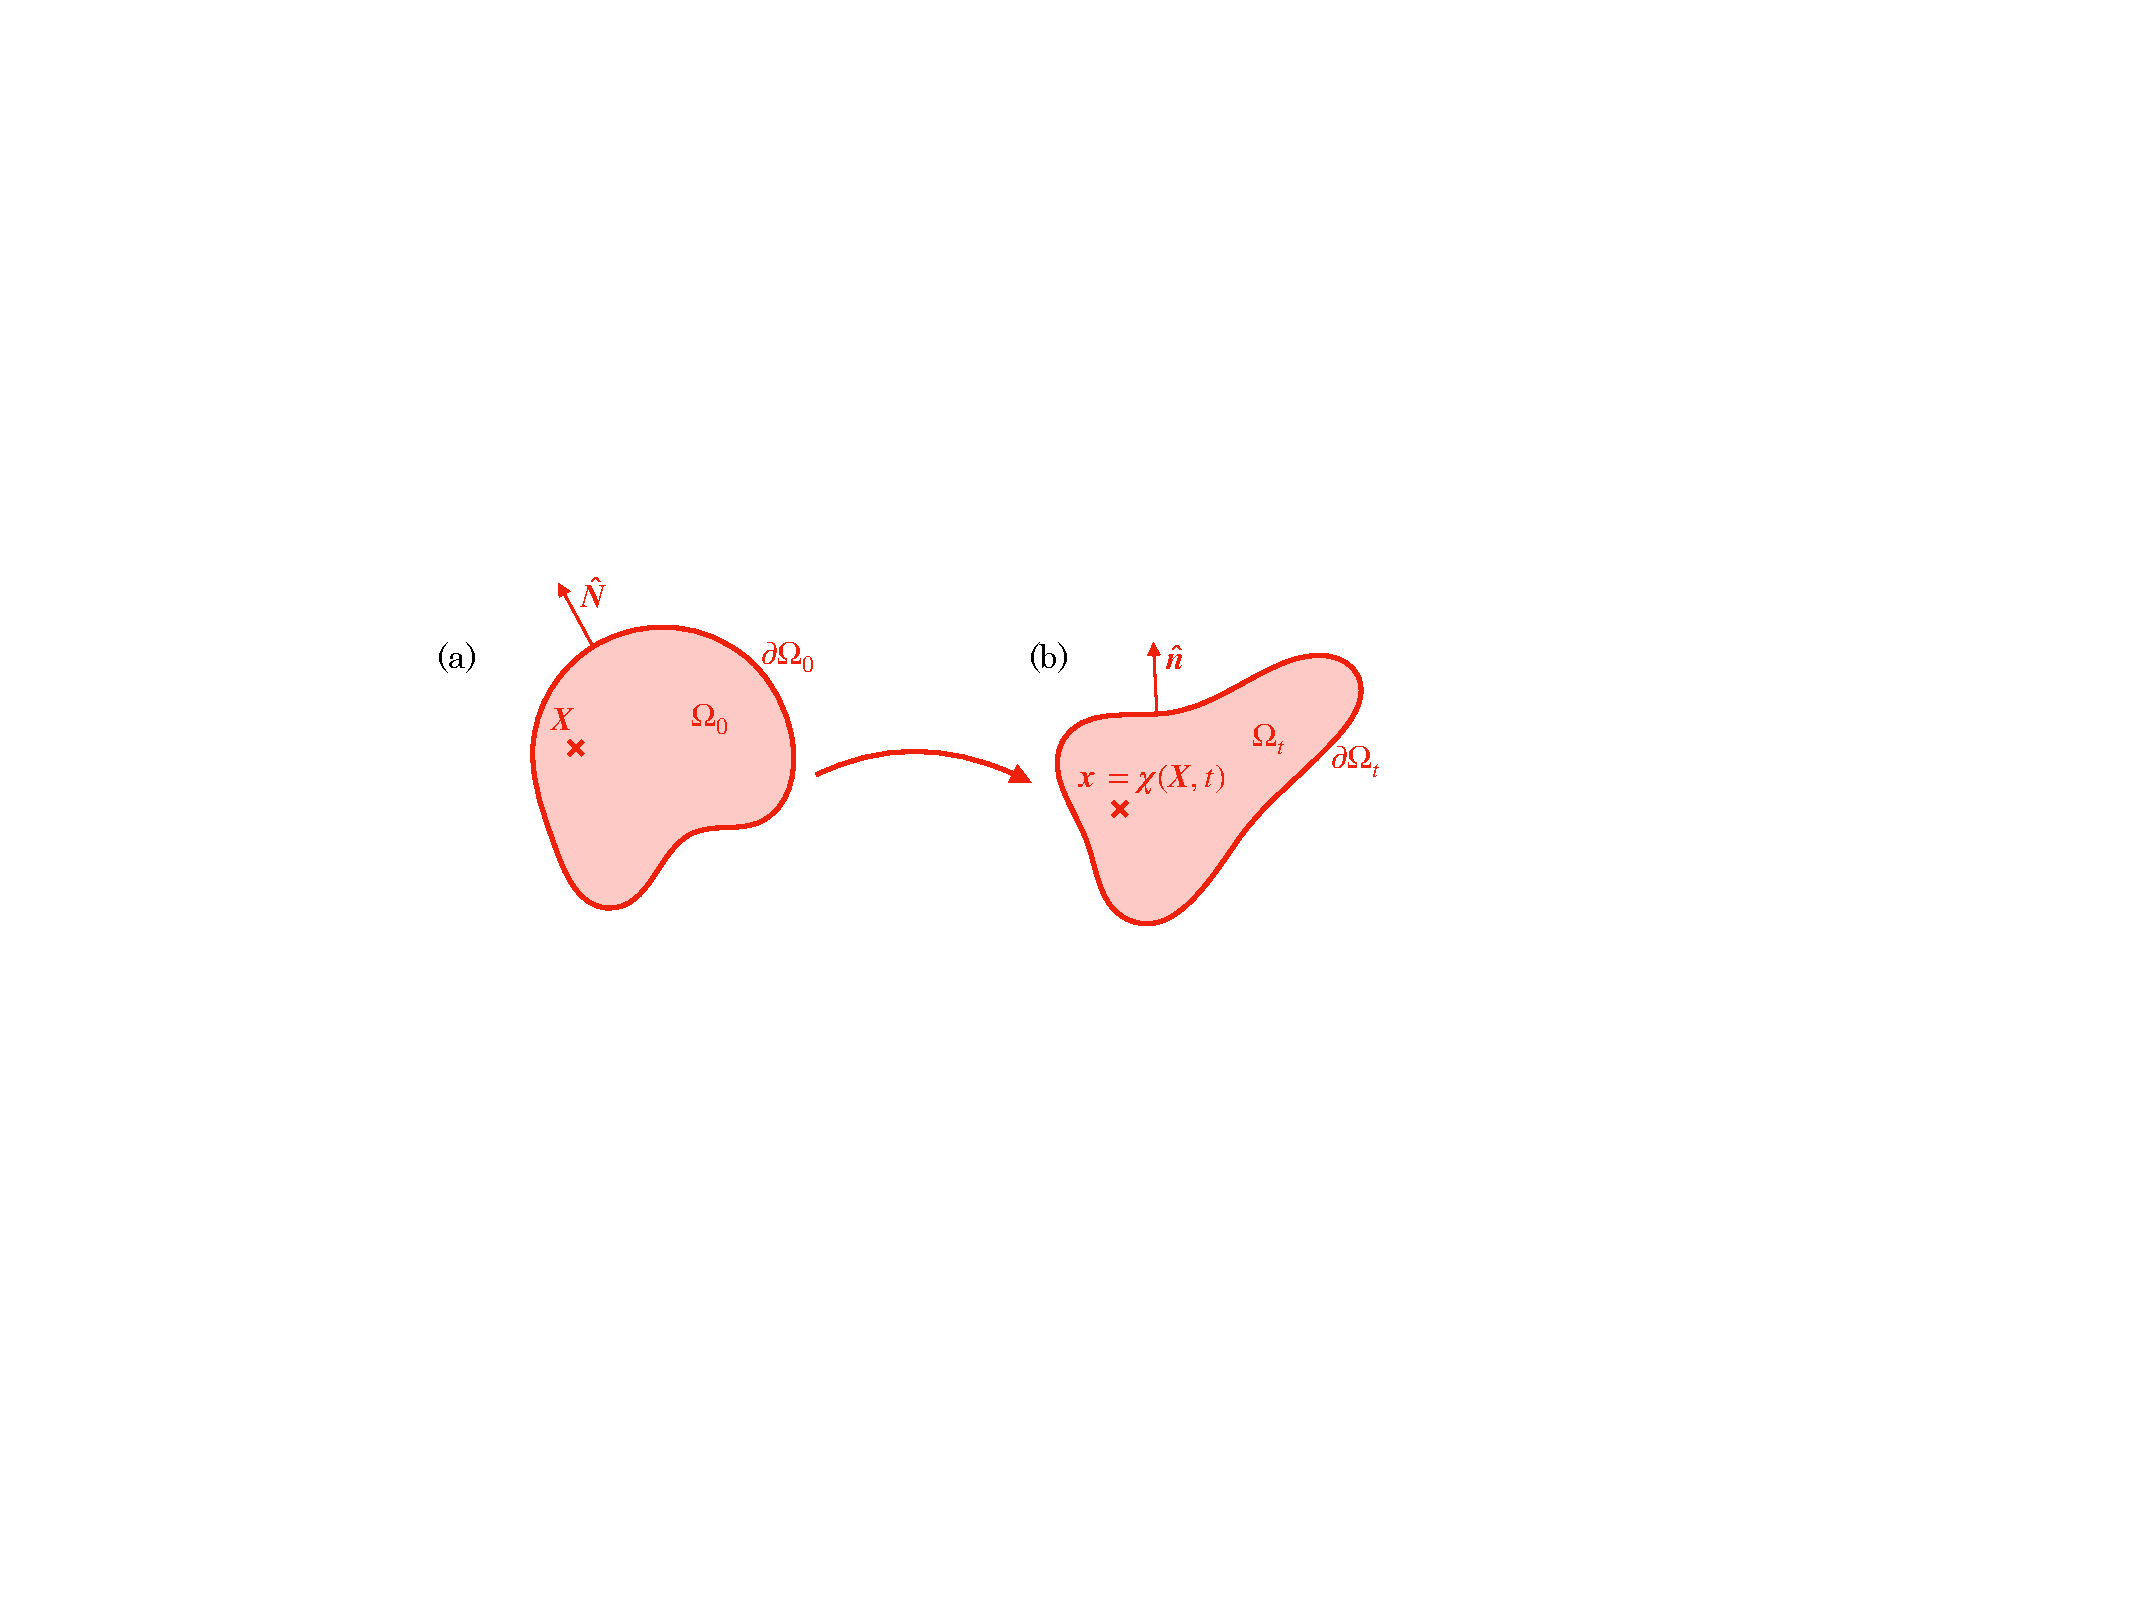
\includegraphics[scale=0.60]{./Figures/Fig1}
\caption{Representation of the body in (a) the reference configuration and (b) the deformed configuration. }
\label{fig:elastic_deformations}
\end{center}
\end{figure}

The material is assumed hyperelastic, so that the second Piola–Kirchhoff stress tensor $\tS$ derives from a strain energy density $W(\tE)$ as $\tS = \partial W/\partial\tE$, where $\tE = (\tF^\top\cdot\tF - \tI)/2$ is the Green--Lagrange strain tensor. 
The simplest hyperelastic model is the Saint Venant--Kirchhoff model, which coincides with classical linear elasticity in the limit of infinitesimal strain, but, being formulated in terms of $\tE$, it remains frame-invariant under arbitrarily large rotations and displacements.

The outward unit normals to the body surface in the reference and deformed configurations are denoted $\bN(\bX)$ and $\bn(\bx)$, respectively. 
The first Piola–Kirchhoff stress tensor $\tP = \tF\cdot\tS$ provides the traction $\bF_s$ in the reference configuration: $\bF_s = \tP\cdot\bN$ is the force per unit reference area exerted on a surface element with outward normal $\bN$, so that the surrounding fluid exerts a force $\bF_s$ on the body. 

%%%%%%%%%%%%%%%%
%\subsubsection{Static equilibrium}
Our goal is to determine the velocity field $\bxd$ of the body in terms of the applied forces and its elastic properties. At low Reynolds number, inertia is negligible and the body is in quasi-static equilibrium at each instant. The equilibrium equations in the reference configuration are
\begin{eqnarray}
\nabla_{\bX}\cdot \tP + \bF_v & = & 0, \quad \mbox{in }\Omega_0,\\
\tP \cdot \bN & = & \bF_s, \quad \mbox{on }\partial\Omega_0,
\end{eqnarray}
expressing the balance of body forces $\bF_v$ against the divergence of the first Piola–Kirchhoff stress, and the continuity of traction at the solid--fluid interface.

To obtain a weak formulation of the equilibrium equations, we apply the principle of virtual power: for any kinematically admissible virtual velocity field $\bV^*(\bX)$, the internal virtual power equals the power of the external forces
\begin{equation}\label{eq:virtual_power}
\int_{\Omega_0} \tS : \tEd^* \, \rmd V =
	\int_{\Omega_0} \bF_v \cdot \bV^* \, \rmd V +
	\int_{\partial \Omega_0} \bF_s \cdot \bV^* \, \rmd S,
\end{equation}
where the virtual strain rate $\tEd^*$ is obtained by differentiating $\tE = (\tF^\top\cdot\tF - \tI)/2$ along the virtual motion
\begin{equation}\label{eq:virtual_strain_rate}
\tEd^* = \sym\left(\tF^\top \cdot \nabla \bV^* \right).
\end{equation}

%%%%%%%%%%%%%%%%
%\subsubsection{Body forces}
We assume that the body force is linear in an externally applied field $\bH$, uniform at the scale of the body,
\begin{equation}
\bF_v(\bx) = \rho(\bx)\,\tC_H(\bx) \cdot \bH
            = \rho_0(\bX)\,\tF \cdot \tC_H(\bX) \cdot \tF^{-1} \cdot \bH,
\end{equation}
where $\tC_H(\bx)$ is a configuration-dependent coupling tensor. The second equality uses $\rho = \rho_0/J$ and the pushforward of $\tC_H$ to the reference configuration. This parameterization covers gravity ($\bH = \bg$, $\tC_H = \tI$) and magnetic forces ($\bH = \bB$, $\tC_H = [\bmu]_\times$, where $\bmu$ is the magnetic moment per unit mass).

%%%%%%%%%%%%%%%%%%%%%%%%%%%%%%%%%%%%%%
\subsection{Fluid}

%%%%%%%%%%%%%%%%
%\subsubsection{Hydrodynamic forces}
The fluid occupies the exterior domain $\bar\Omega_t$ and its motion satisfies the Stokes equations,
\begin{eqnarray}
\nabla p & = & \mu \nabla^2 \bu, \quad \mbox{in }\bar\Omega_t,\\
\nabla \cdot \bu & = & 0, \quad \mbox{in }\bar\Omega_t,
\end{eqnarray}
with $\mu$ the dynamic viscosity and $p$ the pressure field.
We introduce two Stokes solutions that share the same geometry but differ in their boundary conditions on $\partial\Omega_t$ (Fig.~\ref{fig:two_stokes}). The physical solution $(\bu, p)$ represents the disturbance flow due to the moving body; the total fluid velocity is $\bu + \bu^\infty$, with boundary condition
\begin{equation}
\bu = \bxd - \bu^\infty \quad \mbox{on }\partial\Omega_t.
\end{equation}
The auxiliary solution $(\bu^*, p^*)$ is driven by the virtual velocity field,
\begin{equation}
\bu^* = \bV^* \quad \mbox{on }\partial\Omega_t.
\end{equation}

\begin{figure}[t]
\begin{center}
    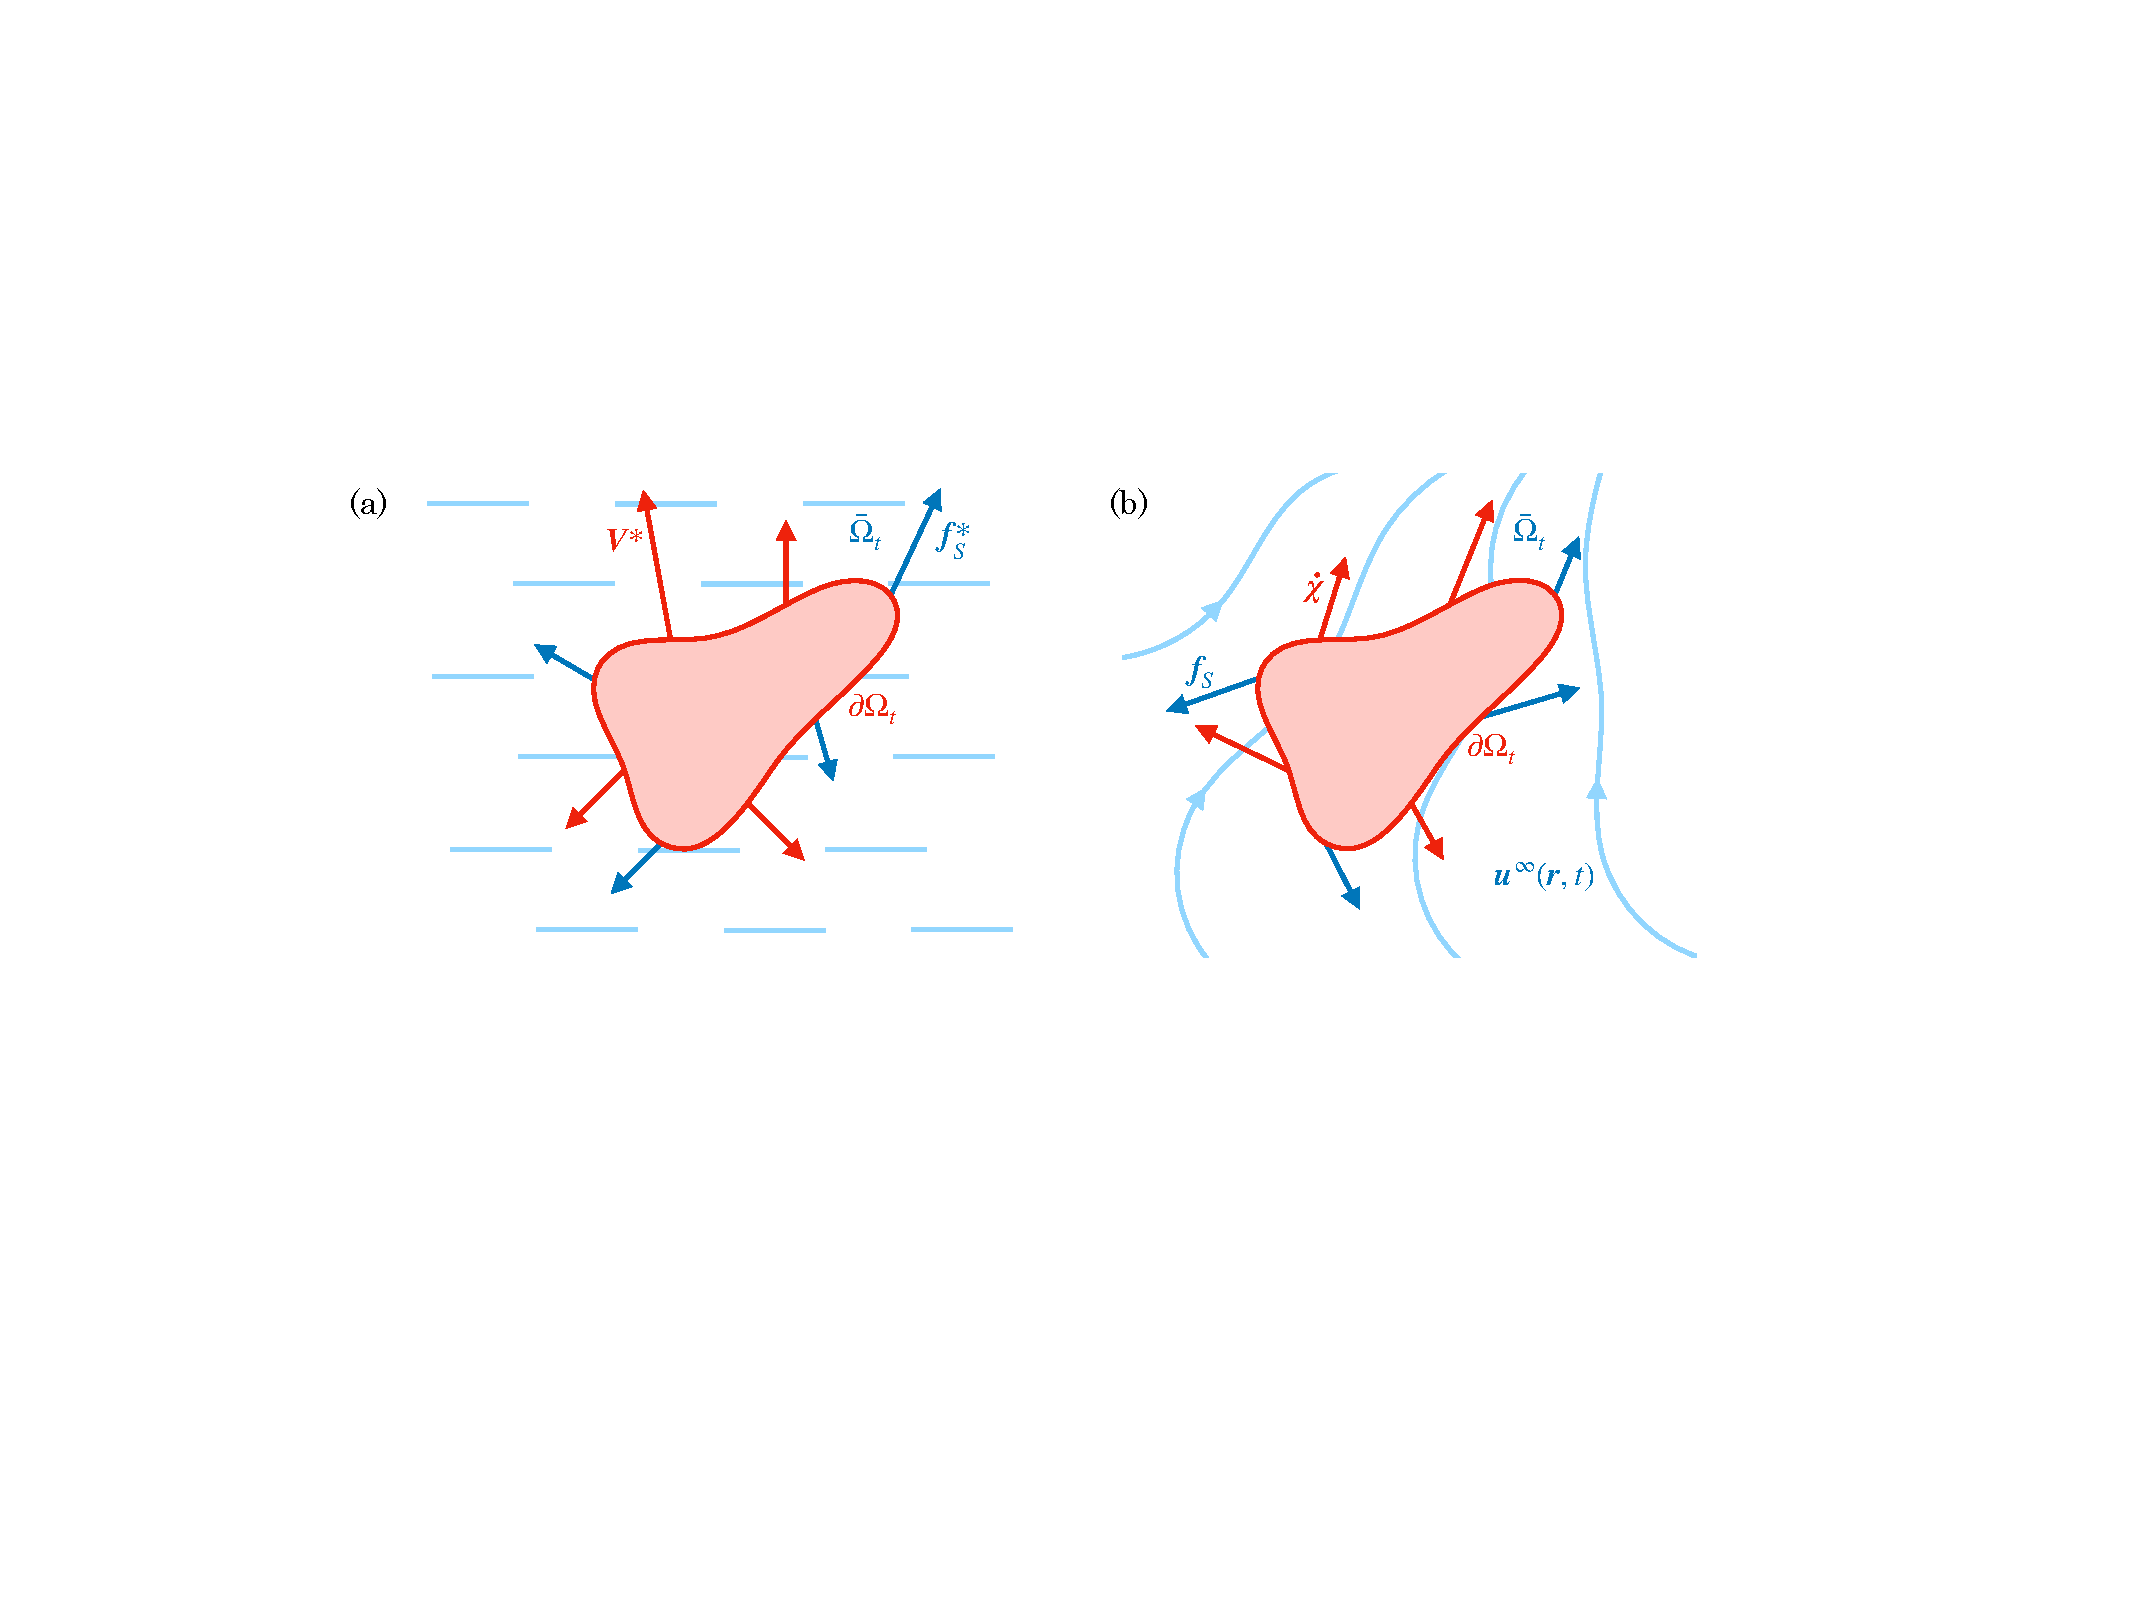
\includegraphics[scale=0.60]{./Figures/Fig2}
\caption{Two solutions of the Stokes equations used in the reciprocal theorem: (a) the auxiliary problem, driven by virtual surface velocity $\bV^*$ in an otherwise quiescent fluid, producing traction $\bff_s^*$ on the left-hand side of Eq.~(\ref{eq:reciprocity}); (b) the physical problem, the body moving with velocity $\bxd$ in background flow $\bu^\infty$, producing traction $\bff_s$ on the right-hand side of Eq.~(\ref{eq:reciprocity}).}
\label{fig:two_stokes}
\end{center}
\end{figure}

Each solution produces a traction on the body surface: $\bff_s$ for the physical flow and $\bff_s^*$ for the virtual flow. Applying the Lorentz reciprocal theorem \cite{Happel2012} to these two Stokes flows gives
\begin{equation}\label{eq:reciprocity}
\int_{\partial \Omega_t} \bff_s \cdot \bV^* \, \rmd s = 
\int_{\partial \Omega_t} \bff_s^* \cdot \left(
										 \bxd - \bu^\infty
									\right) \, \rmd s.
\end{equation}

These integrals in the deformed configuration can also be expressed in the reference configuration using the surface Jacobian $J_s$ (Eq.~\ref{eq:surface_Jacobian})
\begin{equation}
\int_{\partial \Omega_t} \bff_s \cdot \bV^* \, \rmd s =
\int_{\partial \Omega_0} \bF_s \cdot \bV^* \, \rmd S,
\end{equation}
with $\bF_s = J_s\bff_s$ (and similarly $\bF_s^* = J_s\bff_s^*$) the surface force in the reference configuration. We recognize here the last term of Eq. \eqref{eq:virtual_power}, which can thus conveniently be calculated through the following equality
\begin{equation}\label{eq:reciprocity_ref}
\int_{\partial \Omega_0} \bF_s \cdot \bV^* \, \rmd S=
\int_{\partial \Omega_0} \bF^*_s \cdot \left(
										 \bxd - \bu^\infty
									\right) \, \rmd S.
\end{equation}
But to do that, we need to calculate the virtual traction $\bF_s^* = J_s \bff_s^*$ for a body of shape $\bx$ with surface velocity $\bV^*$. From the linearity of the Stokes equations, we know that the relation between $\bff_s^*$ and $\bV^*$ is linear, but depends nonlinearly on the shape $\bx$. In general, $\bF_s^*$ can be computed through the boundary integral equation (Appendix \ref{sec:BIE}). 



%%%%%%%%%%%%%%%%%%%%%%%%%%%%%%%%%%%%%%
\subsection{Summary}
Using Eqs. (\ref{eq:virtual_power}), (\ref{eq:reciprocity}), and (\ref{eq:reciprocity_ref}), we find the weak formulation of the problem on the space $V$ of kinematically admissible velocity fields: one seeks $\bxd\in V$ satisfying 
\begin{equation}\label{eq:weak_form}
\int_{\partial \Omega_0} \bxd  \cdot \bF_s^*\, \rmd S =
	\int_{\partial \Omega_0}   \bu^\infty \cdot \bF_s^* \, \rmd S + 
	\int_{\Omega_0} \tS : \tEd^* \, \rmd V -
	\int_{\Omega_0} \bF_v \cdot \bV^* \, \rmd V,
\end{equation}
for all virtual velocities $\bV^*\in V$.

The left-hand side is linear in the unknown $\bxd$ but nonlinear in the body's shape. The right-hand side is independent of $\bxd$ and is composed of three terms: (1) the virtual power of the viscous forces due to the background flow, (2) the virtual elastic power, and (3) the virtual power of the body forces.

The structure of Eq.~(\ref{eq:weak_form}) becomes transparent through the decomposition of $\bxd$ into a rigid-body part and a strain-producing deformation part. Let $\bu_0$, $\bomega_0$ be the translational and rotational velocity of the body frame. Then
\begin{equation}\label{eq:velocity_decomp}
\bxd(\bX,t) = \bu_0 + \bomega_0\times\left(\bchi(\bx,t)-\br_0\right) + \bV_\mathrm{def}(\bX,t),
\end{equation}
where $\bV_\mathrm{def}$ is the velocity due to shape only.
Two structural consequences follow. First, for any rigid-body virtual velocity $\bV^* = \bu_0^* + \bomega_0^*\times\left(\bchi(\bx,t)-\br_0\right)$, the hyperelastic term in Eq.~(\ref{eq:weak_form}) vanishes. This is because  $\tF^\top \cdot \nabla \bV^*$ is then skew-symmetric in Eq.~(\ref{eq:virtual_strain_rate}) when $\nabla\bV^* = [\bomega_0^*]_\times\cdot\tF$.
Second, comparing Eq.~(\ref{eq:velocity_decomp}) with the background flow linearization~(\ref{eq:bg_flow}), the same operator couples $\bu_0$ and $\bomega_0$ on the left of Eq.~(\ref{eq:weak_form}) and $\bv_0^\infty$ and $\bomega_0^\infty$ on the right. Only the relative velocities $(\bu_0 - \bu_0^\infty)$ and $(\bomega_0 - \bomega_0^\infty)$ therefore drive the hydrodynamic coupling. This is consistent with Galilean invariance.


%%%%%%%%%%%%%%%%%%%%%%%%%%%%%%%%%%%%%%%%%%%%%%%%%%%%%%%%%%%%%%%%%%%%%%%%%%%%%
\section{Numerical approaches\label{sec.numerics}}


Inverting Eq. \eqref{eq:weak_form} allows one to compute $\bxd$ and thus to simulate through time integration the transport and deformation of a soft body in a background flow. 
The difficulty is that all operators depend on the current shape. An efficient method would be to project the deformation onto a set of discrete meaningful modes, for instance, by computing the least attenuated viscous eigenmodes of the system with no background flow and no body forces (Appendix~\ref{sec:Galerkin}). 
An alternative is to consider a soft body made of rigid spheres connected by springs, as done below. 


%%%%%%%%%%%%%%%%%%%%%%%%%%%%%%%%%%%%%%
\subsection{Kinematics of a sphere assembly\label{sec.kinematics}}

We consider an assembly of $N$ spheres connected by springs and rods.  The $i$-th sphere of radius $a_i$ has center position $\bR_i$ and Rodrigues orientation vector $\bTheta_i$ in the body frame $(\bE_1,\bE_2,\bE_3)$. 
Both are gathered in a six-component position $\bX_i(\bQ,t)$, a function of time and the $N_Q$ degrees of freedom $\bQ$ representing the deformation (Fig.~\ref{fig:assembly_spheres}). 
The associated six-component velocity is $\bV_i = [\bU_i, \bOmega_i]$, with $\bU_i$ the translational velocity and $\bOmega_i$ the angular velocity.  
The  six-component velocity $\bV_i$ is related to $\bQd$ by the per-sphere Jacobian $\tJ_i = \partial \bV_i/\partial \bQd$ 
\begin{equation}
\bV_i = \tJ_i \cdot \bQd + (\bV_\mathrm{act})_i,
\end{equation}
with $(\bV_\mathrm{act})_i = \tB_6 \cdot \partial\bX_i/\partial t$ an active component due to prescribed kinematics and $\tB_6(\bTheta_i)$ the Bortz operator (see Appendix~\ref{app:bortz}).

Stacking all spheres, the grand velocity $\bV = [\bV_1, \dots, \bV_N]$ in the body frame satisfies
\begin{equation}\label{eq.Jacobian_assembly}
\bV = \tJ_\mathrm{sph} \cdot \bQd + \bV_\mathrm{act},
\end{equation}
with the grand active velocity $\bV_\mathrm{act} = [(\bV_\mathrm{act})_1, \dots, (\bV_\mathrm{act})_N]$ of size $6N$ collecting the per-sphere contributions, and the assembly Jacobian $\tJ_\mathrm{sph}(\bQ,t) = \partial \bV/\partial \bQd$ of size $6N \times N_Q$. 
Because $\bV$ is affine in $\bQd$, it is a quasi-velocity of the Lagrangian system.

\begin{figure}[t]
\begin{center}
    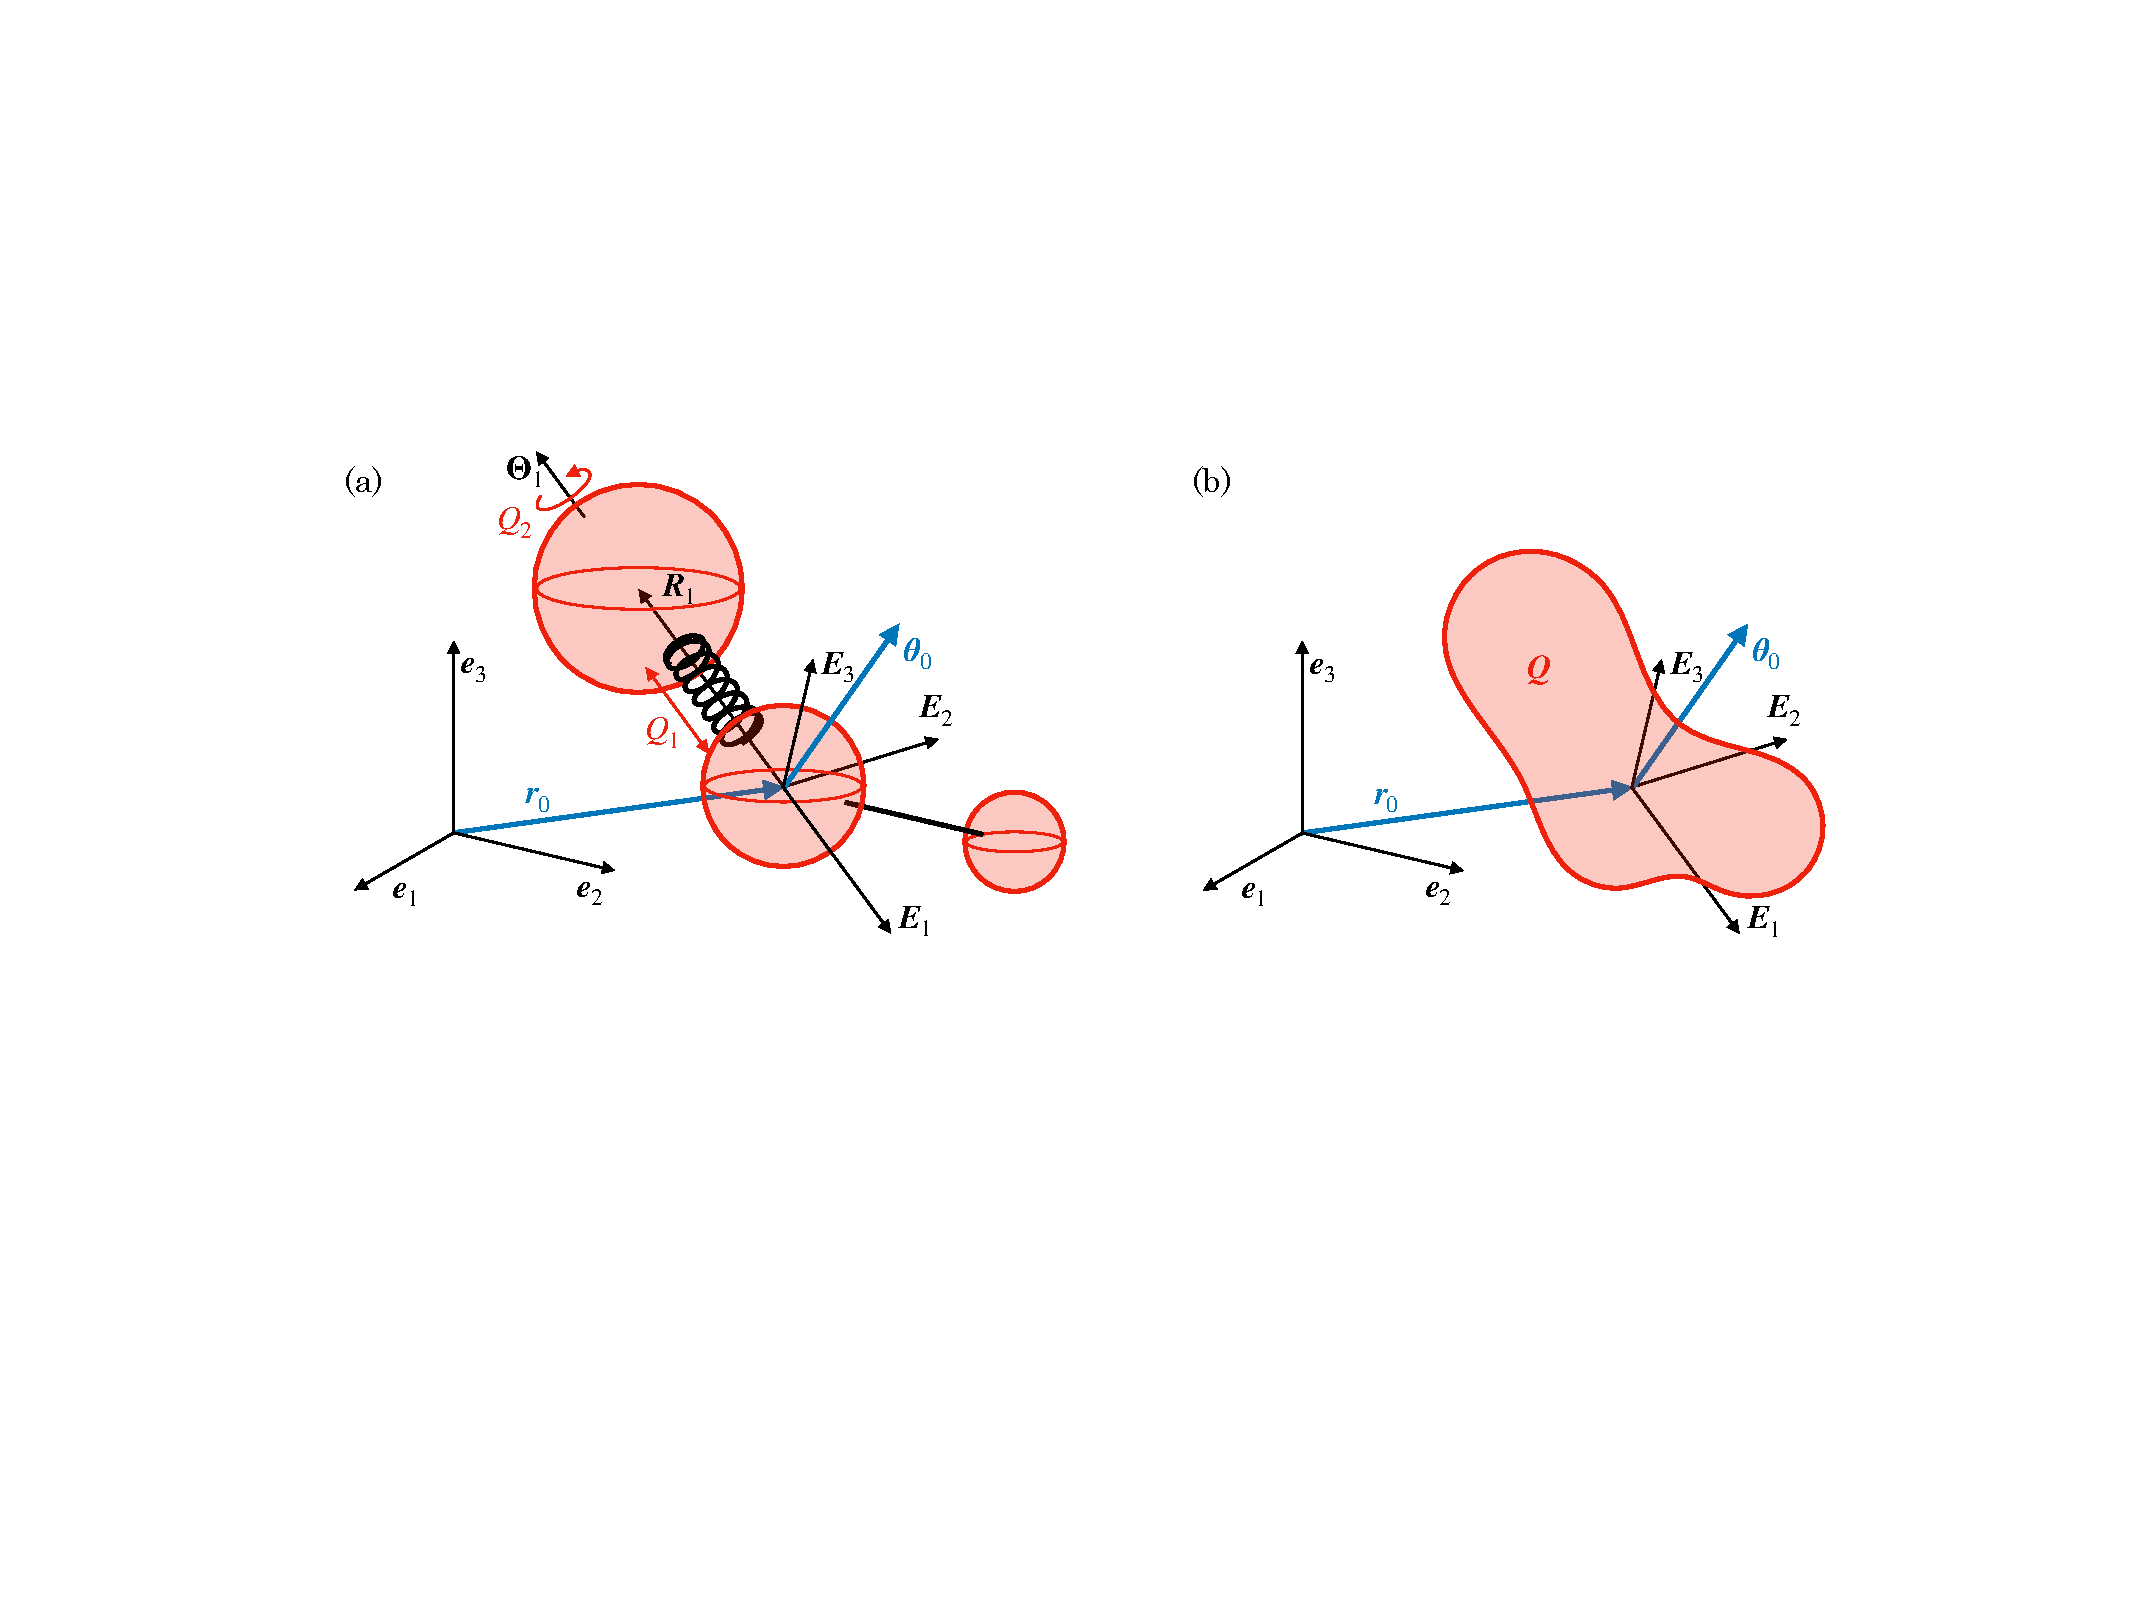
\includegraphics[scale=0.60]{./Figures/Fig3}
\caption{Notations for an assembly of spheres.
(a) Assembly of $N=3$ spheres with $N_Q=2$ degrees of freedom $\bQ=[Q_1,Q_2]$. In the assembly frame, the $i$-th sphere is at position $\bR_i$ and has an orientation $\bTheta_i$. The assembly frame is at position $\br_0$ and orientation $\btheta_0$ in the laboratory frame.
(b) The assembly configuration is entirely represented by its position $\br_0$, its orientation $\btheta_0$, and its degrees of freedom $\bQ$.}
\label{fig:assembly_spheres}
\end{center}
\end{figure}

The body's frame $(\bE_1,\bE_2,\bE_3)$ undergoes a global rigid-body motion.
Its position and orientation are encoded in the six-component position $\bx_0 = [\br_0, \btheta_0]$, where $\br_0$ is the position and $\btheta_0$ the Rodrigues orientation of the body's frame. 
The full state of the assembly in the laboratory frame is therefore given by the generalized coordinates (of size $N_q = 6 + N_Q$)
\begin{equation}
\bq = \left[\bx_0,\, \bQ \right].
\end{equation}
We also define the six-component velocity $\bv_0 = [\bu_0, \bomega_0]$, with $\bu_0$ the translational velocity and $\bomega_0$ the angular velocity of the body in the laboratory frame. 
This six-component velocity is  associated with a generalized velocity
\begin{equation}
\bp = \left[\bu_0,\, \bomega_0,\, \bQd \right] = \tB(\btheta_0) \cdot \bqd,
\end{equation}
where $\tB(\btheta_0)$ is a $N_q\times N_q$ Bortz matrix given in Appendix~\ref{app:bortz}. 

The laboratory-frame velocity of sphere $i$ combines the body-frame velocity $\bV_i$ with the rigid-body transport due to $\bv_0$:
$$\bu_i = \bU_i + \bu_0 + \bomega_0 \times \bR_i, \quad \bomega_i = \bOmega_i + \bomega_0.$$
Stacking all spheres, this composition takes the compact form
\begin{equation}\label{eq.composition_velocities}
\bv = \bV + \tC_U \cdot \bv_0 = \bV + \tC_U \cdot \tB_6 \cdot \bm{\dot x}_0,
\end{equation}
with $\tB_6(\btheta_0)$ the Bortz operator evaluated at the body-frame orientation and $\tC_U$ a $6N\times 6$ transport coupling tensor. Combining Eqs.~(\ref{eq.Jacobian_assembly}) and (\ref{eq.composition_velocities}), the grand velocity of all spheres in the laboratory frame is related to $\bp$ by
\begin{equation}\label{eq.U_is_J_Qdot}
\bv = \bV_\mathrm{act} + \tJ \cdot \bp = \bV_\mathrm{act} + \tJ \cdot \tB \cdot \bqd,
\end{equation}
where $\tJ = \partial \bv/\partial \bp$ is the $6N\times N_q$ full Jacobian. Because $\tB$ is invertible, the grand sphere velocities $\bv$ are quasi-velocities of this Lagrangian system.

The linearized background flow [Eq.~(\ref{eq:bg_flow})] evaluated at the sphere centers gives the grand flow velocity $\bv^\infty = [\bv^\infty_1,\dots,\bv^\infty_N]$ and the rate-of-strain tensor
\begin{equation}\label{eq:grandflowvelocity}
\bv^\infty = \tC_U \cdot \bv_0^\infty + \tC_S : \tE_0^\infty, \quad \tE^\infty = \tE_0^\infty,
\end{equation}
where $\tC_U$ is the same transport coupling tensor as in Eq.~(\ref{eq.composition_velocities}) and $\tC_S$ is a $6N\times 3\times 3$ stresslet coupling tensor. Here $\bv_0^\infty = [\bu_0^\infty, \bomega_0^\infty]$ denotes the six-component velocity of the undisturbed flow evaluated at the reference point $\br_0$. For simplicity, we also introduce the generalized flow velocity $\bp_0^\infty = [\bu_0^\infty, \bomega_0^\infty, \mathbf{0}]$ of size $N_q=6+N_Q$. 


%%%%%%%%%%%%%%%%%%%%%%%%%%%%%%%%%%%%%%
\subsection{Soft mobility equation of a sphere assembly}

With the kinematic description established, we now derive the equation of motion by applying the principle of virtual power to the sphere assembly. We then show how to reduce it to the soft mobility equation.

The six-component force $\bff_i = [\bF_i, \bT_i]$ acting on sphere $i$ collects the force $\bF_i$ applied at its center and the associated torque $\bT_i$. Stacking all forces into the  grand force $\bff = [\bff_1,\dots,\bff_N]$, it can be decomposed as
$$\bff = \bff_c + \bff_\mathrm{hydro} + \bff_\mathrm{ext} + \bff_K,$$
where $\bff_c$ are internal constraint forces (maintaining prescribed inter-sphere constraints), $\bff_\mathrm{hydro}$ are hydrodynamic forces, $\bff_\mathrm{ext}$ are external body forces, and $\bff_K$ are elastic restoring forces. The elastic forces are linear in the deformation state,
\begin{equation}\label{eq.linear_elasticity}
\bff_K = \tC_K \cdot \bQ,
\end{equation}
and satisfy $\sum_{i=1}^N (\bff_K)_i = 0$ (Newton's third law for internal forces). The body forces are linear in an external field $\bH$,
\begin{equation}\label{eq.body_force}
\bff_\mathrm{ext} = \tC_H \cdot \bH.
\end{equation}

The principle of virtual power allows us to eliminate the unknown constraint forces. For any virtual velocity $\bv^*$ compatible with the constraints, the constraint forces do not work and hence $\bff_c \cdot \bv^* = 0$. The virtual power of all forces can thus be written:
\begin{equation}
P^* = \left(\bff_\mathrm{hydro} + \bff_\mathrm{ext} + \bff_K\right) \cdot \bv^* = 0,
\end{equation}
and it vanishes because the forces balance. 
Since $\bv^* = (\partial \bv/\partial \bp)\cdot \bp^*$,
and the above equality must hold for all $\bp^*$, one obtains
\begin{equation}\label{eq.generalized_force_Q}
\tJ^\top \cdot \left(\bff_\mathrm{hydro} + \bff_\mathrm{ext} + \bff_K\right) = 0,
\end{equation}
where $\tJ = \partial \bv/\partial \bp$ is the same Jacobian as in Eq.~(\ref{eq.U_is_J_Qdot}). This projection, deduced from classical tools of Lagrangian mechanics, reduces the $6N$-dimensional force balance to the $N_q$ dimensions of the generalized coordinates while eliminating the constraint forces $\bff_c$ from the equations of motion.


The hydrodynamic force on the sphere assembly is given by the grand resistance relation
\begin{equation}\label{eq.mobility_problem_all_spheres}
\bff_\mathrm{hydro} = \tR \cdot \left( \bv^\infty - \bv \right) + \tR_S : \tE^\infty,
\end{equation}
where $\tR$ is the $6N\times 6N$ grand resistance matrix and $\tR_S$ is the $6N\times 3\times 3$ stresslet resistance tensor. 

Substituting Eqs.~(\ref{eq.U_is_J_Qdot}), (\ref{eq:grandflowvelocity}), and (\ref{eq.mobility_problem_all_spheres}) into the generalized force balance~(\ref{eq.generalized_force_Q}) and writing $\bff = \bff_\mathrm{ext} + \bff_K$ for the non-hydrodynamic forces gives
\begin{equation}
\left(\tJ^\top \cdot \tR \cdot \tJ\right) \cdot \bp  =  \tJ^\top \cdot \left[\bff - \tR\cdot\bV_\mathrm{act} + \tR \cdot \bv^\infty + \tR_S : \tE^\infty \right],
\end{equation}
Because $\tR$ is symmetric positive definite and $\tJ$ has full column rank, $\tJ^\top \cdot \tR \cdot \tJ$ is invertible. Introducing the $N_q\times 6N$ projection operator
\begin{equation}\label{eq:projection}
\tPi = \left( \tJ^\top \cdot \tR \cdot \tJ \right)^{-1} \cdot \tJ^\top \cdot \tR,
\end{equation}
which satisfies $\tPi \cdot \tJ = \tI$, the system can be put in the compact form
\begin{equation}\label{eq:soft_mobility}
\bp = \tM \cdot \bff - \tPi \cdot \bV_\mathrm{act} + \bp_0^\infty + \tC_E : \tE_0^\infty,
\end{equation}
with the soft mobility and flow-coupling tensors
\begin{equation}\label{eq:soft_tensors}
\tM = \tPi \cdot \tR^{-1} = \left(\tJ^\top \cdot \tR \cdot \tJ\right)^{-1} \cdot \tJ^\top, \quad
\tC_E = \tPi \cdot (\tC_S + \tR^{-1} \cdot \tR_S).
\end{equation}
The tensor $\tM$ of size $N_q\times 6N$ extends the classical rigid-body mobility to deformable assemblies, the projection $\tPi$ eliminates the constraint forces from the equations of motion by retaining only the components of the $6N$-dimensional force balance that are compatible with the kinematic Jacobian $\tJ$.


Substituting the force decompositions~(\ref{eq.linear_elasticity})--(\ref{eq.body_force}) yields
\begin{equation}\label{eq.MK_MH}
\tM \cdot \bff_K = \tM_K \cdot \bQ, \quad \tM \cdot \bff_\mathrm{ext} = \tM_H \cdot \bH,
\end{equation}
with $\tM_K = \tM \cdot \tC_K$ of size $N_q\times N_Q$ and $\tM_H = \tM \cdot \tC_H$ of size $N_q\times 3$.

Equation~(\ref{eq:soft_mobility}) constitutes the soft mobility equation of the assembly. Expressed in the body's frame, it reads
\begin{equation}\label{eq:soft_mobility_body}
\bp - \bp_0^\infty = 
\left(
\begin{array}{c}
\bu_0 - \bu_0^\infty\\[0.5ex]
\bomega_0 - \bomega_0^\infty\\[0.5ex]
\bQd
\end{array}
\right) =
  \tM_K \cdot \bQ + \tM_H \cdot \bH + \tC_E : \tE_0^\infty - \tPi \cdot \bV_\mathrm{act},
\end{equation}
where $\tM_K$, $\tM_H$, $\tC_E$, and $\tPi$ depend only on the deformation state $\bQ$. 
The four right-hand-side terms admit a clean physical reading. 
The elastic mobility $\tM_K = \tM\cdot\tC_K$ (size $N_q \times N_Q$) carries the response to internal elastic forces. The body-force mobility $\tM_H = \tM\cdot\tC_H$ (size $N_q \times 3$) carries the response to the external field $\bH$ (gravity, magnetic). 
The flow-coupling tensor $\tC_E$ (size $N_q \times 3\times 3$) is the soft-body analogue of the Bretherton tensor and couples the body to the background rate-of-strain. 
The last term $-\tPi\cdot\bV_\mathrm{act}$ projects any prescribed kinematics of the spheres (active actuation) onto the generalized coordinates. The left-hand side is the deviation of the generalized velocity from the rigid-body part of the background flow: only relative velocities couple, consistent with Galilean invariance.

Since $\bp = \tB^{-1}\cdot\bqd$, Eq.~\eqref{eq:soft_mobility_body} is a first-order ODE of the form $\bqd = f(\bq, t)$, which can be integrated forward in time given initial conditions and the prescribed flow and external fields. 
When the flow and external fields are known in the laboratory frame, they must be rotated into the body's frame before evaluating the right-hand side:
\begin{equation}\label{eq:rotation_fields}
\bu_0^\infty = \mRot^\top \cdot \left(\bu_0^\infty\right)_\mathrm{lab}, \quad
\tE_0^\infty = \mRot^\top \cdot \left(\tE_0^\infty\right)_\mathrm{lab} \cdot \mRot, \quad
\bH = \mRot^\top \cdot \left(\bH \right)_\mathrm{lab},
\end{equation}
where $\mRot(\btheta_0)$ is the rotation matrix given by the Euler--Rodrigues formula~(\ref{eq:Rodrigues_formula}).

%%%%%%%%%%%%%%%%%%%%%%%%%%%%%%%%%%%%%%
\subsection{Python library}

The soft mobility framework for sphere assemblies is implemented in \emph{softmobility}, a Python library freely available as open-source code \cite{softmobility}. The library is organized around four capabilities, each illustrated by tutorials.

First, a sphere assembly is constructed by declaring its spheres (radii, positions, orientations, forces, torques) symbolically in terms of three classes of variables: degrees of freedom $\bQ$, design parameters $\btheta$ (stiffnesses, rest lengths, radii) targeted by optimization, and external inputs (fields and active controls). A parser imports these spheres from a YAML file and linearises the symbolic forces in the inputs to build the coupling matrices $\tC_K$ and $\tC_H$ of Eqs.~(\ref{eq.linear_elasticity}) and (\ref{eq.body_force}).

Second, given the design parameters $\btheta$ and the current degrees of freedom $\bQ$, the library computes all the soft mobility tensors of Eq.~(\ref{eq:soft_mobility_body}). The grand resistance matrix $\tR$ is computed from the Rotne--Prager--Yamakawa approximation, the projection $\tPi$, and the reduced tensors $\tM_K$, $\tM_H$, $\tC_E$ are computed automatically, without the user assembling Jacobians or coupling tensors by hand.

Third, the trajectory of the soft body is integrated forward in time with a fourth-order Runge--Kutta scheme, given a prescribed background flow, external fields (gravity, magnetic field), and any active kinematics. Anchored bodies (clamped fibers) are handled through the mixed mobility system of Appendix~\ref{app:clamped_anchor}.

Fourth, all numerical operations are implemented in JAX \cite{jax2018github}, making the entire rollout just-in-time compilable and end-to-end differentiable. This enables gradient-based optimization of shape and stiffness parameters $\btheta$ via the Optax library \cite{optax2020github}: any scalar objective of the trajectory (e.g., average swim speed) can be maximized or minimized by automatic differentiation through the simulation.


%%%%%%%%%%%%%%%%%%%%%%%%%%%%%%%%%%%%%%%%%%%%%%%%%%%%%%%%%%%%%%%%%%%%%%%%%%%%%
\section{Results\label{sec.results}}

The proposed framework is illustrated on five canonical problems organized along two axes: increasing complexity of the body (rigid $\to$ soft) and of its environment (quiescent fluid $\to$ background flow), followed by design optimization. 
These five problems are proposed as example notebooks in the \emph{softmobility} library \cite{softmobility} (all figures below are generated by these notebooks).  


%%%%%%%%%%%%%%%%%%%%%%%%%%%%%%%%%%%%%%
\subsection{Sinking of a rigid body}
To test our numerical implementation for non-trivial rigid body dynamics in a quiescent fluid, we first consider the gravity-driven sinking of a rigid four-sphere assembly.
In that case, the degrees of freedom $\bQ$ are absent, the soft mobility equation~(\ref{eq:soft_mobility}) reduces to a rigid mobility equation. We further assume that the body and fluid set a typical scale $a=1$, a typical weight $mg=1$, and viscosity $\mu=1$. Thus, the problem becomes entirely dimensionless and purely geometrical. 

If the reference point $\br_0$ coincides with the center of mass, such that gravity does not exert a torque on the body, the mobility equation is
\begin{equation}\label{eq:rigid_mobility_body} 
\left(
\begin{array}{c}
	\bu_0 \\[0.5ex]
	\bomega_0 
\end{array}
\right) =
  \tM \cdot 
\left(
\begin{array}{c}
	\bG \\[0.5ex]
	\mathbf{0} 
\end{array}
\right),
\end{equation}
with $\bG$ the unit gravity direction expressed in the body's frame and $\tM$ the $6\times 6$ symmetric rigid-body mobility matrix, also expressed in the body's frame ($\tM$ is also the soft mobility matrix in Eq.~(\ref{eq:soft_tensors}) when the number of degrees of freedom $N_Q$ is zero). The mobility matrix $\tM$ can be written in terms of three $3\times 3$ blocks   
\begin{equation}
\tM = \begin{pmatrix} \ta & \tb^\top \\ \tb & \tc \end{pmatrix}. 
\end{equation}

Furthermore, if the reference point $\br_0$ is at the hydrodynamic center of mobility, the block $\tb$ is symmetric \cite{Kim2013} and the dynamics of $\bG$ in the body's frame can be written~\cite{Gonzalez2004}
\begin{equation}\label{eq:Gdot}
\bGd = -\bomega_0 \times \bG = \bG \times \left( \tb \cdot \bG\right),
\end{equation}
which is similar to the classical problem of a rigid body spinning in a vacuum~\cite{Marsden2013} with the difference that the eigenvalues of $\tb$ are not necessarily positive. The solution to Eq.~(\ref{eq:Gdot}) can be expressed in terms of Jacobi elliptic functions of time in the eigenvector basis of $\tb$~\cite{Marsden2013}. 
This analytical solution serves as a benchmark for the code time integration.
It is interesting to note that Eq.~(\ref{eq:Gdot}) has been rederived several times in the literature in different contexts, but few authors point to its analytical solution \cite{Weinberger1972, Gonzalez2004, Weber2013, Palusa2018, Braverman2020, Witten2020, Miara2024, Huseby2025, Joshi2025}.

The body's geometry is made of four spheres touching each other. It is chiral so that the rotation--translation coupling block of the mobility tensor is non-trivial. In practice, we compute the hydrodynamic center of mobility and then distribute the masses of the four spheres so that the centre of mass coincides with the hydrodynamic mobility centre (Fig.~\ref{fig:sinking_rigid}a). 
We integrate the equation of motion (\ref{eq:rigid_mobility_body}) with our code, which implements a fourth-order Runge--Kutta scheme, with 400 timesteps per period (Fig.~\ref{fig:sinking_rigid}b). The numerical and
analytical trajectories of the unit vector $\bG$ agree to better than numerical precision (Fig.~\ref{fig:sinking_rigid}c--d).

%%%%%%%%%%%%%%%%%
\begin{figure}[t]
\begin{center}
    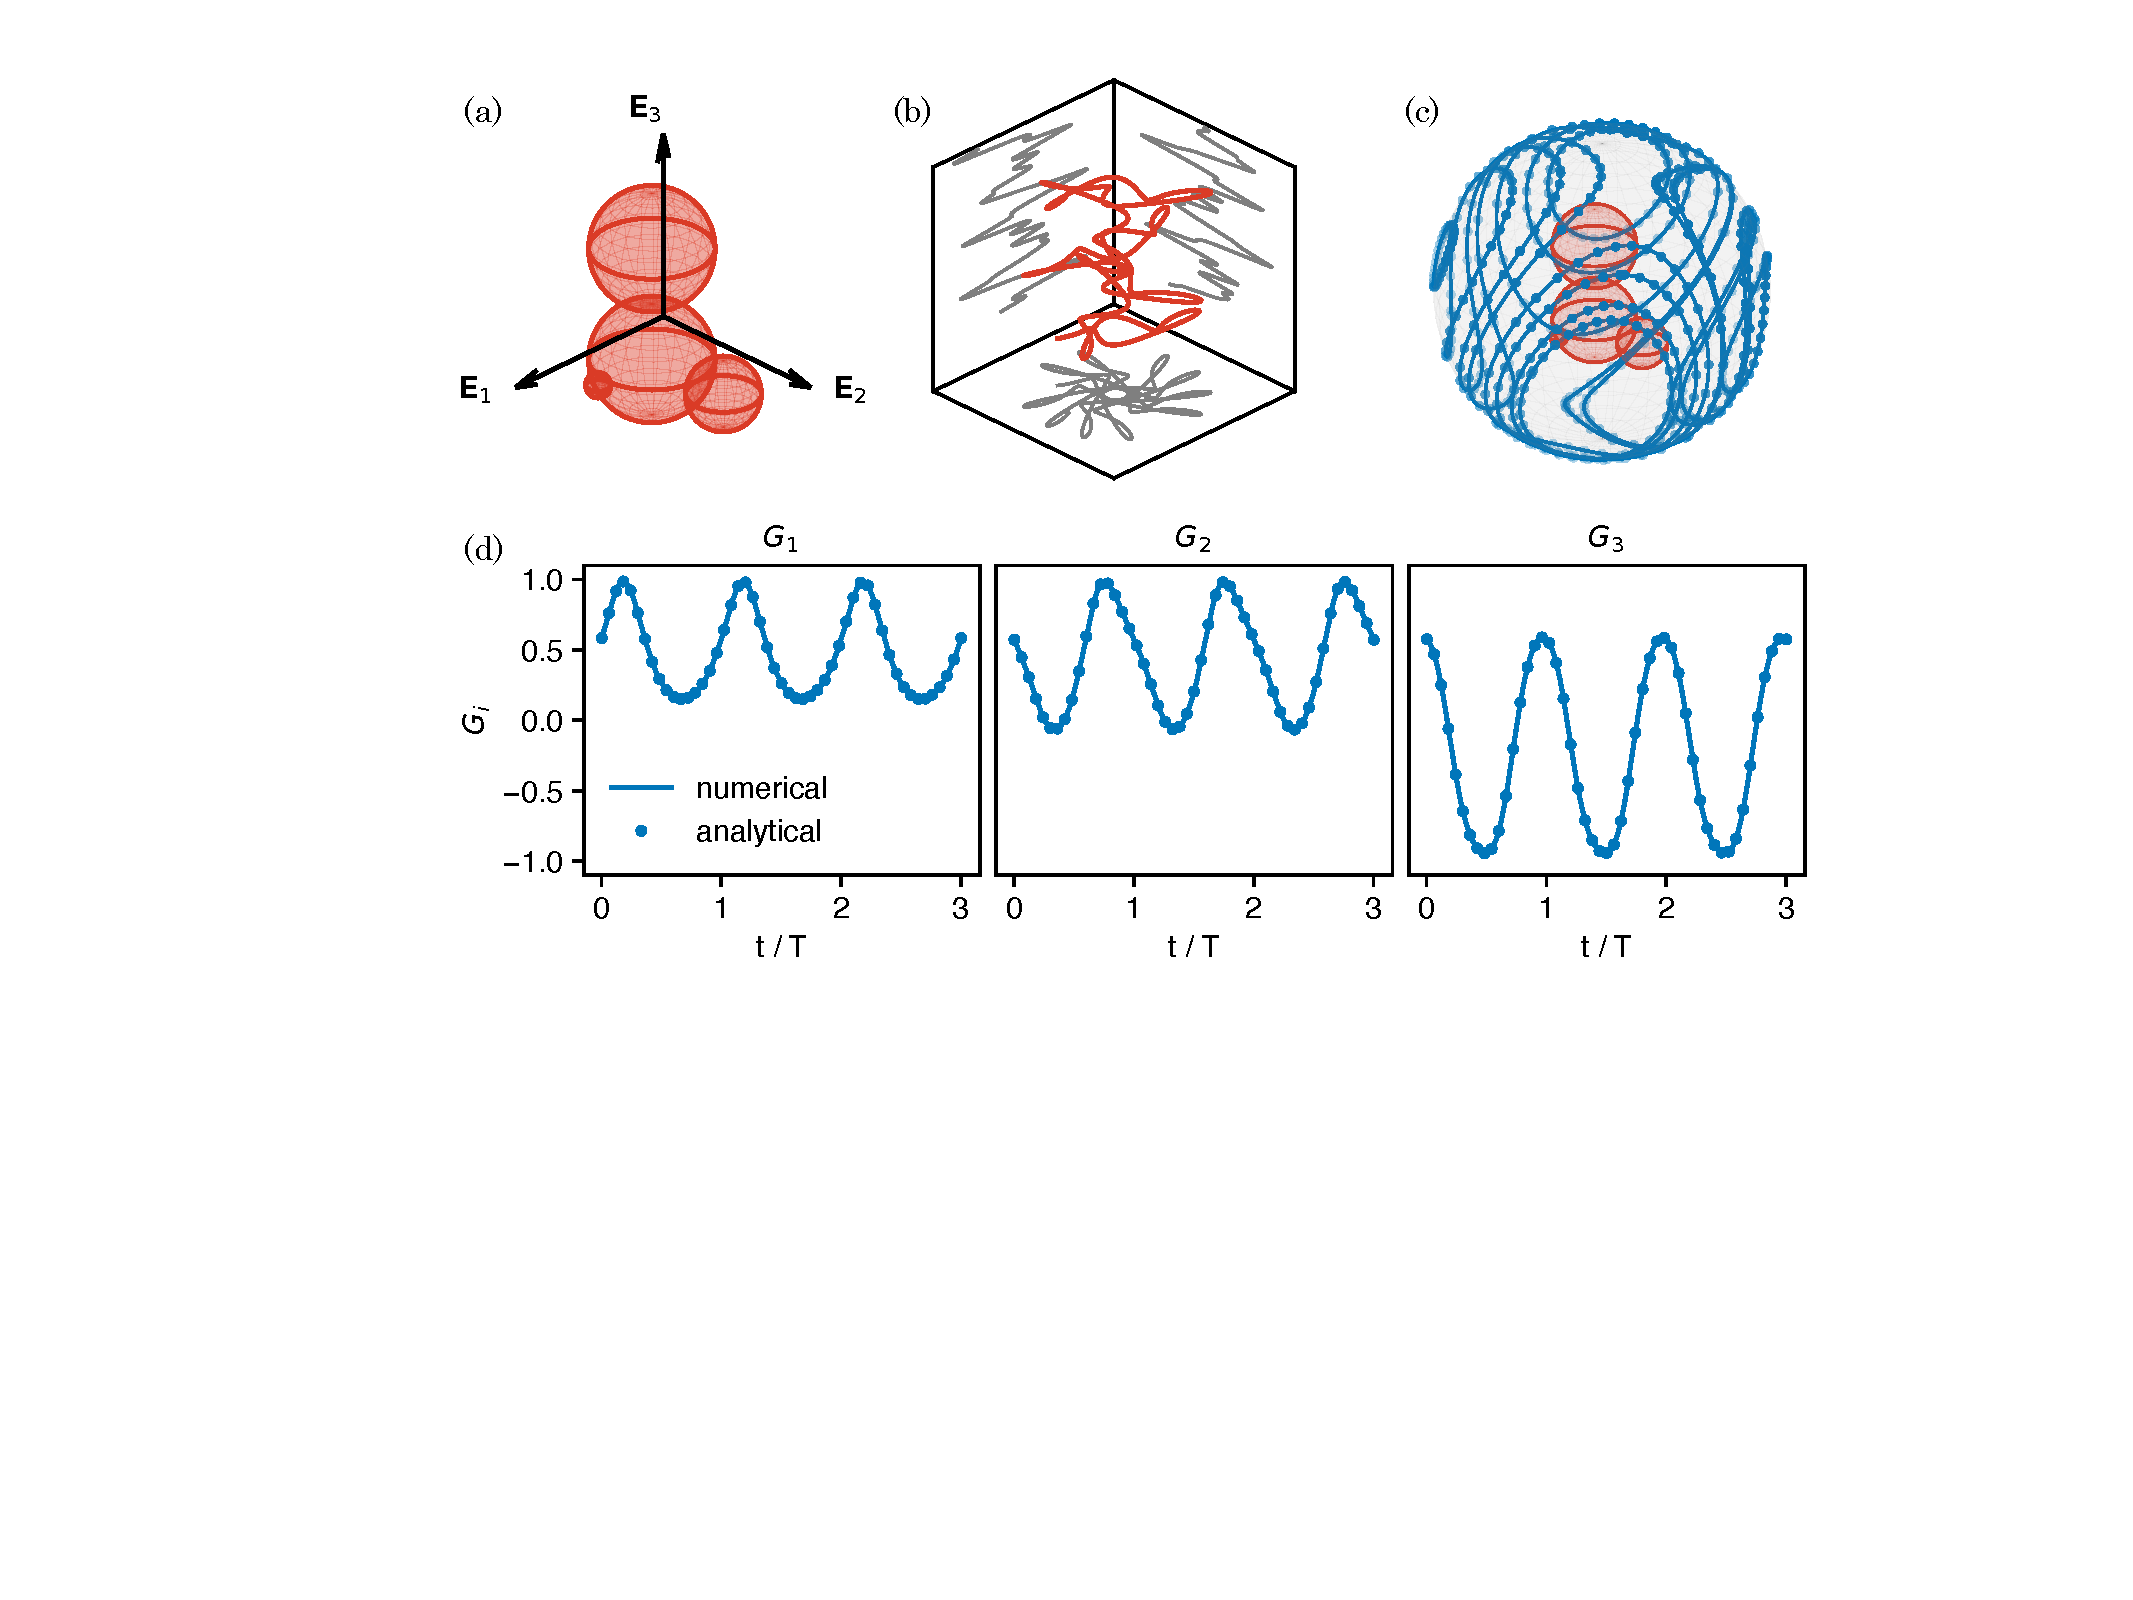
\includegraphics[scale=0.60]{./Figures/Fig4}
\caption{
	Sinking dynamics of a chiral rigid body.
	(a) Geometry of the body, with body's frame $(\bE_1, \bE_2, \bE_3)$ centered on the center of mass (identical to the hydrodynamic center of mobility).
	(b) Example of trajectory $\br_0$ of the center of mass in the laboratory frame (the vertical axis $\be_3$ is compressed by a factor 300). 
	(c) Periodic orbits of the unit gravity vector $\bG$ in the body's frame (lines: simulation, dots: analytical solution). 
	(d) Example of a periodic of orbits: the three components of $\bG$ are shown as a function of time.  
}
\label{fig:sinking_rigid}
\end{center}
\end{figure}
%%%%%%%%%%%%%%%%%

%%%%%%%%%%%%%%%%%%%%%%%%%%%%%%%%%%%%%%
\subsection{Flexible fiber\label{sec:fibers}}

%General fibers
We now want to test the code implementation of elasticity. The most common  deformable object in the literature is a flexible fiber \cite{Du-Roure2019}.
In our case, the fiber is modelled as $N$ touching spheres joined by linear torsional springs of stiffness $k=B/2a$. The parameter $B$ is equivalent to the bending rigidity, such that $B = (\pi/4) E a^4$ for a fiber of radius $a$, with $E$ the Young's modulus. 

%Sinking
We first consider the problem of a negatively buoyant fiber sinking in a fluid at rest. The fiber is modelled with $N=10$ spheres.
The problem is governed by the dimensionless rigidity $\hat B = B / F_\perp L^2$, with $F_\perp = N m g$ the total weight of the fiber, $m$ being the weight of each sphere~\cite{Li2013,Delmotte2015}. 

As the fiber settles under gravity in a quiescent fluid, the problem activates the $N_Q=N-1$ soft degrees of freedom $\bQ$ and the stiffness mobility $\tM_K$ for the first time (Fig.~\ref{fig:sinking_fiber}a). 
Starting from a straight configuration, the fiber relaxes to a steady horseshoe shape (Fig.~\ref{fig:sinking_fiber}b), whose curvature
increases as $\hat B$ decreases (Fig.~\ref{fig:sinking_fiber}c). 
We recover the progression from a nearly straight rod
to a tightly curled U reported in Refs~\cite{Li2013,Delmotte2015} with slight differences due to the different implementations: Li et al.~\cite{Li2013} consider a fiber with elliptic shape, and Delmotte et al.~\cite{Delmotte2015} consider resistive force theory only, which does not include hydrodynamic interactions between the different parts of the fiber. 

%%%%%%%%%%%%%%%%%
\begin{figure}[t]
\begin{center}
    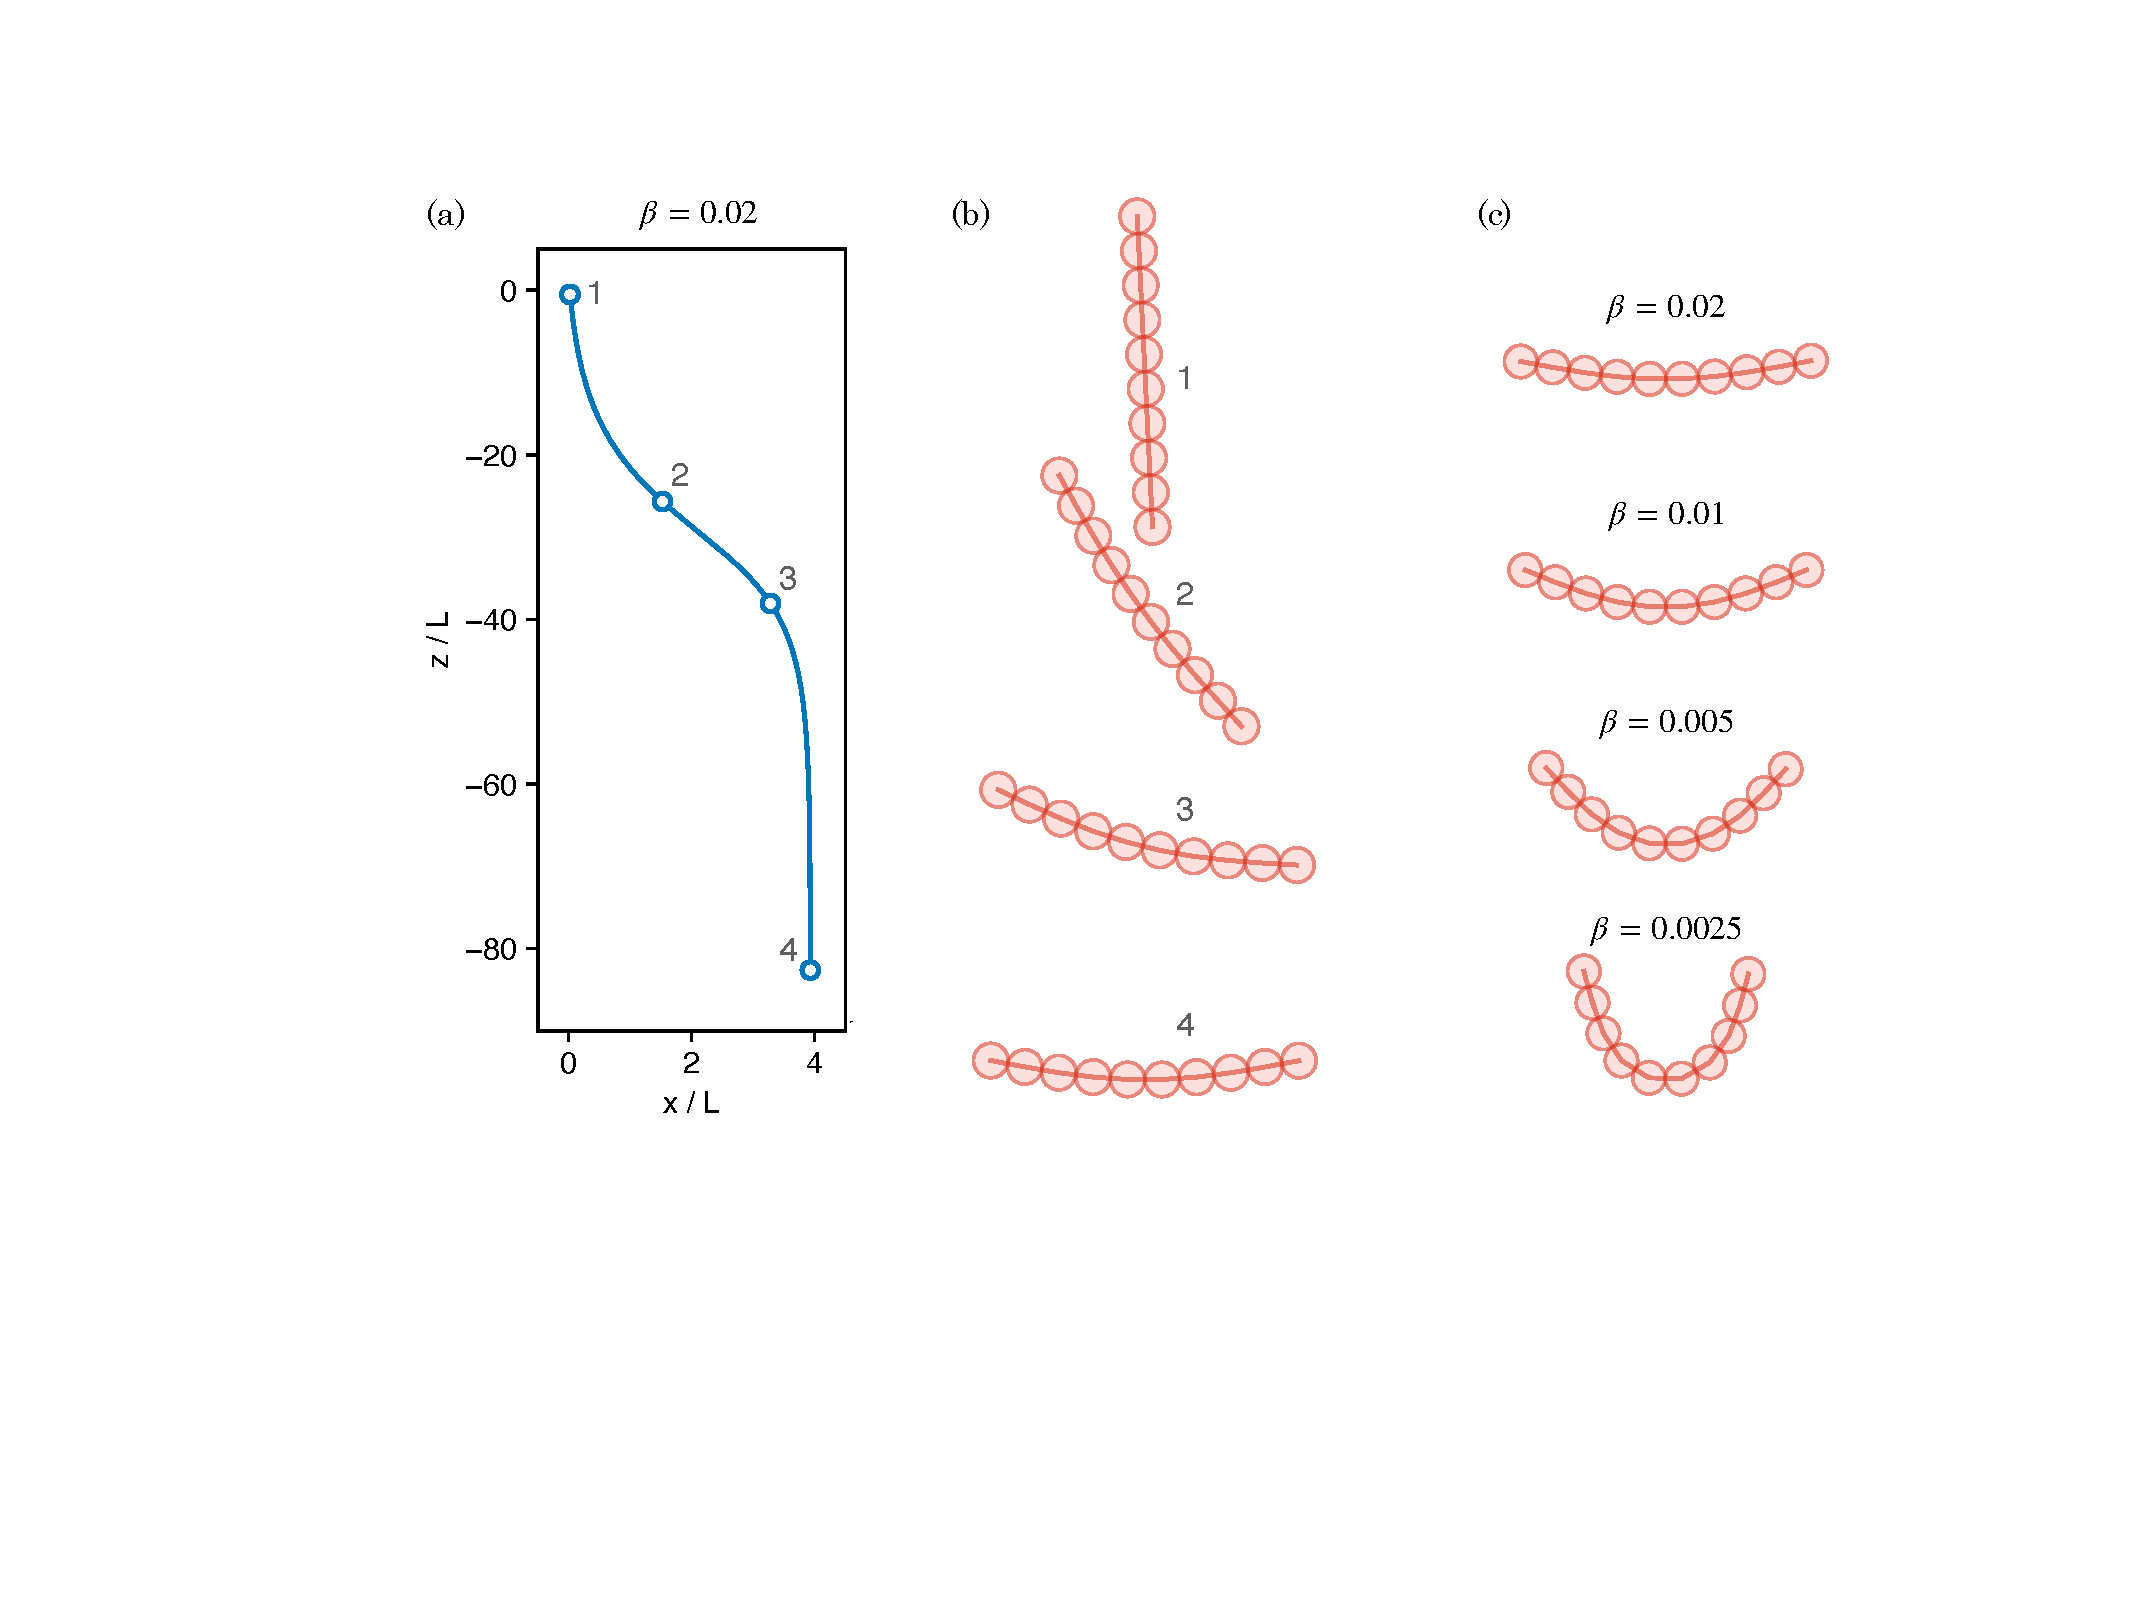
\includegraphics[scale=0.60]{./Figures/Fig5}
\caption{
	Sinking dynamics of a flexible fiber ($N=10$ beads of identical radius $a$).
	(a) For an initial angle of $\pi/32$ with respect to the vertical, the graph shows the position of the center of mass of the fiber in the laboratory frame.  
	(b) Snapshots showing the deformation of the fiber along the trajectory shown in (a). 
	(c) Final shape for fiber of decreasing rigidity as labelled. 
}
\label{fig:sinking_fiber}
\end{center}
\end{figure}
%%%%%%%%%%%%%%%%%

% Rotating
The next case breaks planarity and introduces prescribed kinematics. 
We consider a flexible fiber made of $N=8$ spheres, clamped at one end to an off-axis support
that is forced to rotate around a fixed axis~\cite{Wiggins1998,Coq2008,Coq2009}. 
Assuming infinitely stiff twisting rigidity, this soft body has $N_Q=14$ degrees of freedom (two bending degrees per adjacent sphere pair). 
The clamp acts as a kinematic constraint and generates an unknown reaction force and torque. 
It is handled through a different soft mobility system derived in Appendix~\ref{app:clamped_anchor},
which takes as unknown $\bQd$ and $\bff_0=[\bF_0,\bT_0]$, the force and torque acting on the clamped sphere 0. 

In this problem, the dimensionless control parameter is the Sperm number $\mathrm{Sp} = {L}/{L_\omega}$, with $L_\omega = \left({B}/{\mu_\perp\,\omega}\right)^{1/4}$ and $\mu_\perp = {4\pi\mu}/{\ln(L/a) + 1/2}$, the slender-body transverse drag. 
Our aim is to reproduce the experimental results of Refs~\cite{Coq2008,Coq2009}, in which the fiber is set at an angle $\psi=15^\circ$ with respect to the rotating axis. In these references, the Sperm number is defined with an exponent $4$ compared to the standard definition used here.
As $\mathrm{Sp}^4$ is increased from $0.5$ to $35$, the shape progresses from a nearly straight rotating fiber through a steady three-dimensional shape that progressively wraps onto the rotation axis, reproducing the regimes documented experimentally (Fig.~\ref{fig:rotating_fiber}). 
Steady state is assessed by the body-frame condition $\max\|\bQd\|\,\tau_\mathrm{el}\ll 1$, where $\tau_\mathrm{el} = (2a)^4\mu / B$ is the typical elastic relaxation time.

%%%%%%%%%%%%%%%%%
\begin{figure}[t]
\begin{center}
    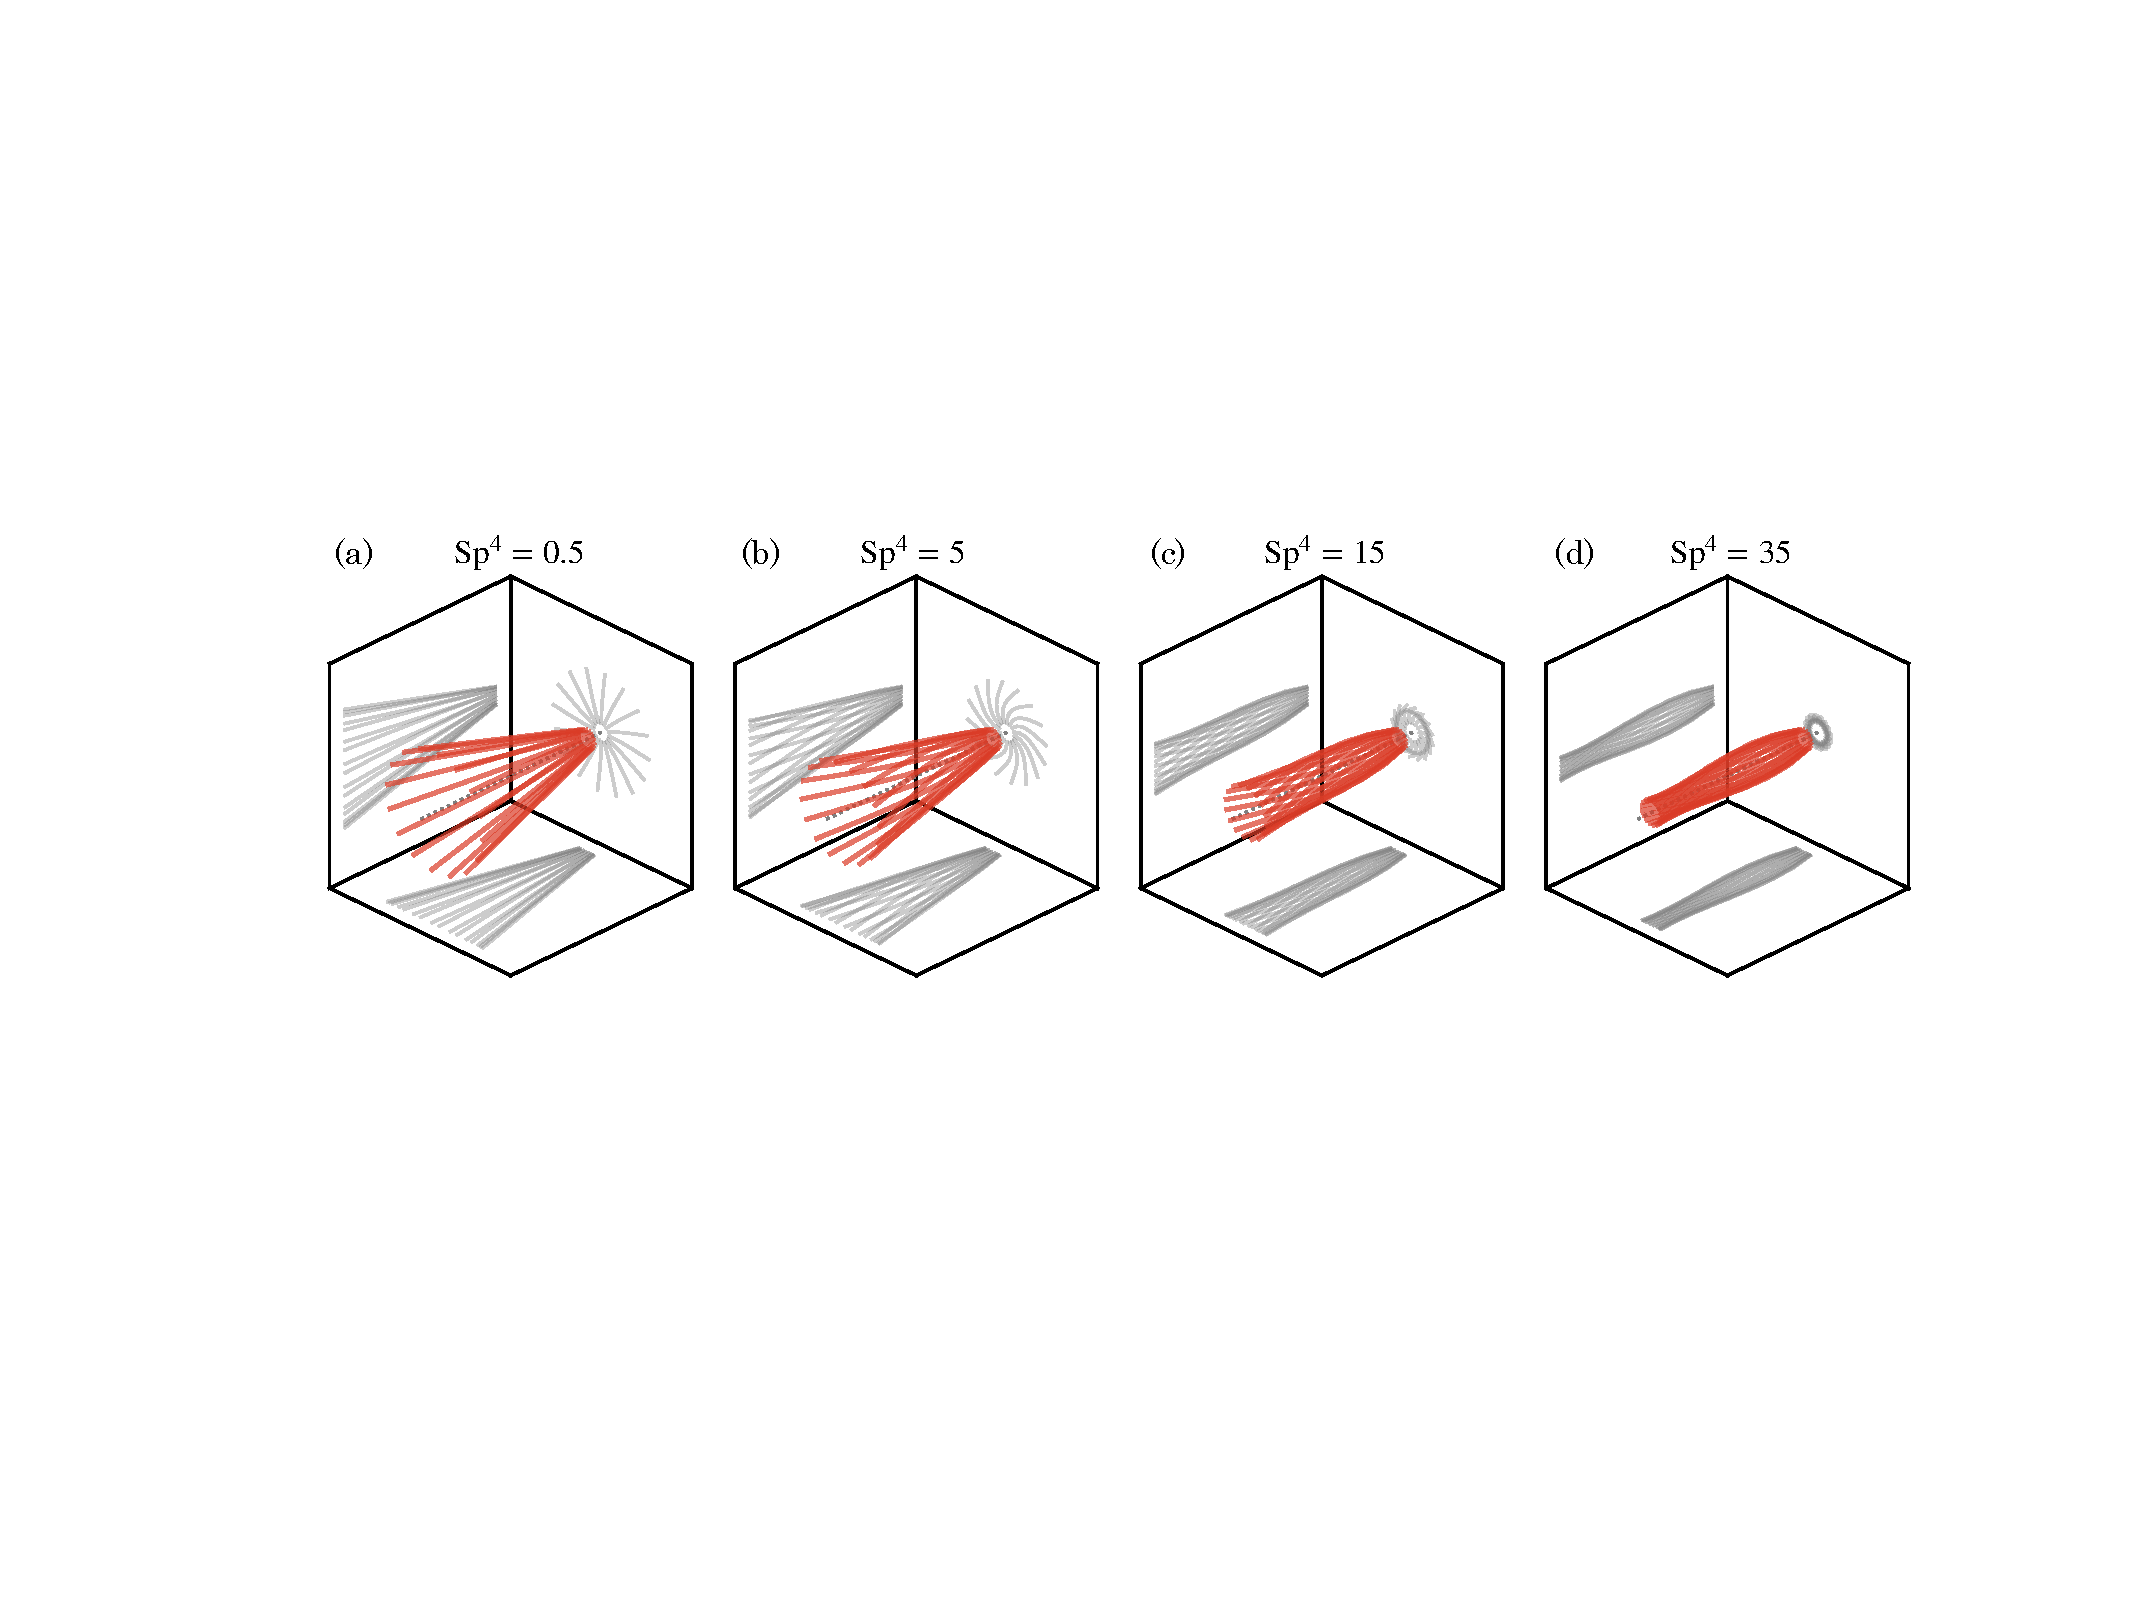
\includegraphics[scale=0.60]{./Figures/Fig6}
\caption{
	Shape of a rotating flexible fiber. 
	The fiber is made of $N=8$ beads and is set at an angle $\psi=15^\circ$ with an offset of $\delta_0/L=0.05$ with respect to the horizontal rotating axis (black line). 
}
\label{fig:rotating_fiber}
\end{center}
\end{figure}
%%%%%%%%%%%%%%%%%

% Tumbling
The third case considers a flexible fiber made of $N=15$ spheres, in a pure shear flow $\bu^\infty = \dot\gamma\,y\,\be_1$. 
To break the symmetry, the fiber has an intrinsic curvature of $\kappa_0=0.01/L$. 
The problem is governed by the dimensionless rigidity $\bar B = B / (8\pi\mu\dot\gamma a^4)$, which compares elastic and viscous forces.
Figure~\ref{fig:tumbling_fiber} shows the tumbling dynamics when $\bar B = 200$: after a short transient, the fiber periodically rotates in the shear plane. Its maximum curvature and its angular velocity both reach a peak when the fiber is normal to the flow direction (C shape numbered 5 in Fig.~\ref{fig:tumbling_fiber}c). 
This tumbling dynamics is similar to what has been reported in experiments~\cite{Liu2018} and simulations~\cite{Schmid2000,Delmotte2015}.

%%%%%%%%%%%%%%%%%
\begin{figure}[t]
\begin{center}
   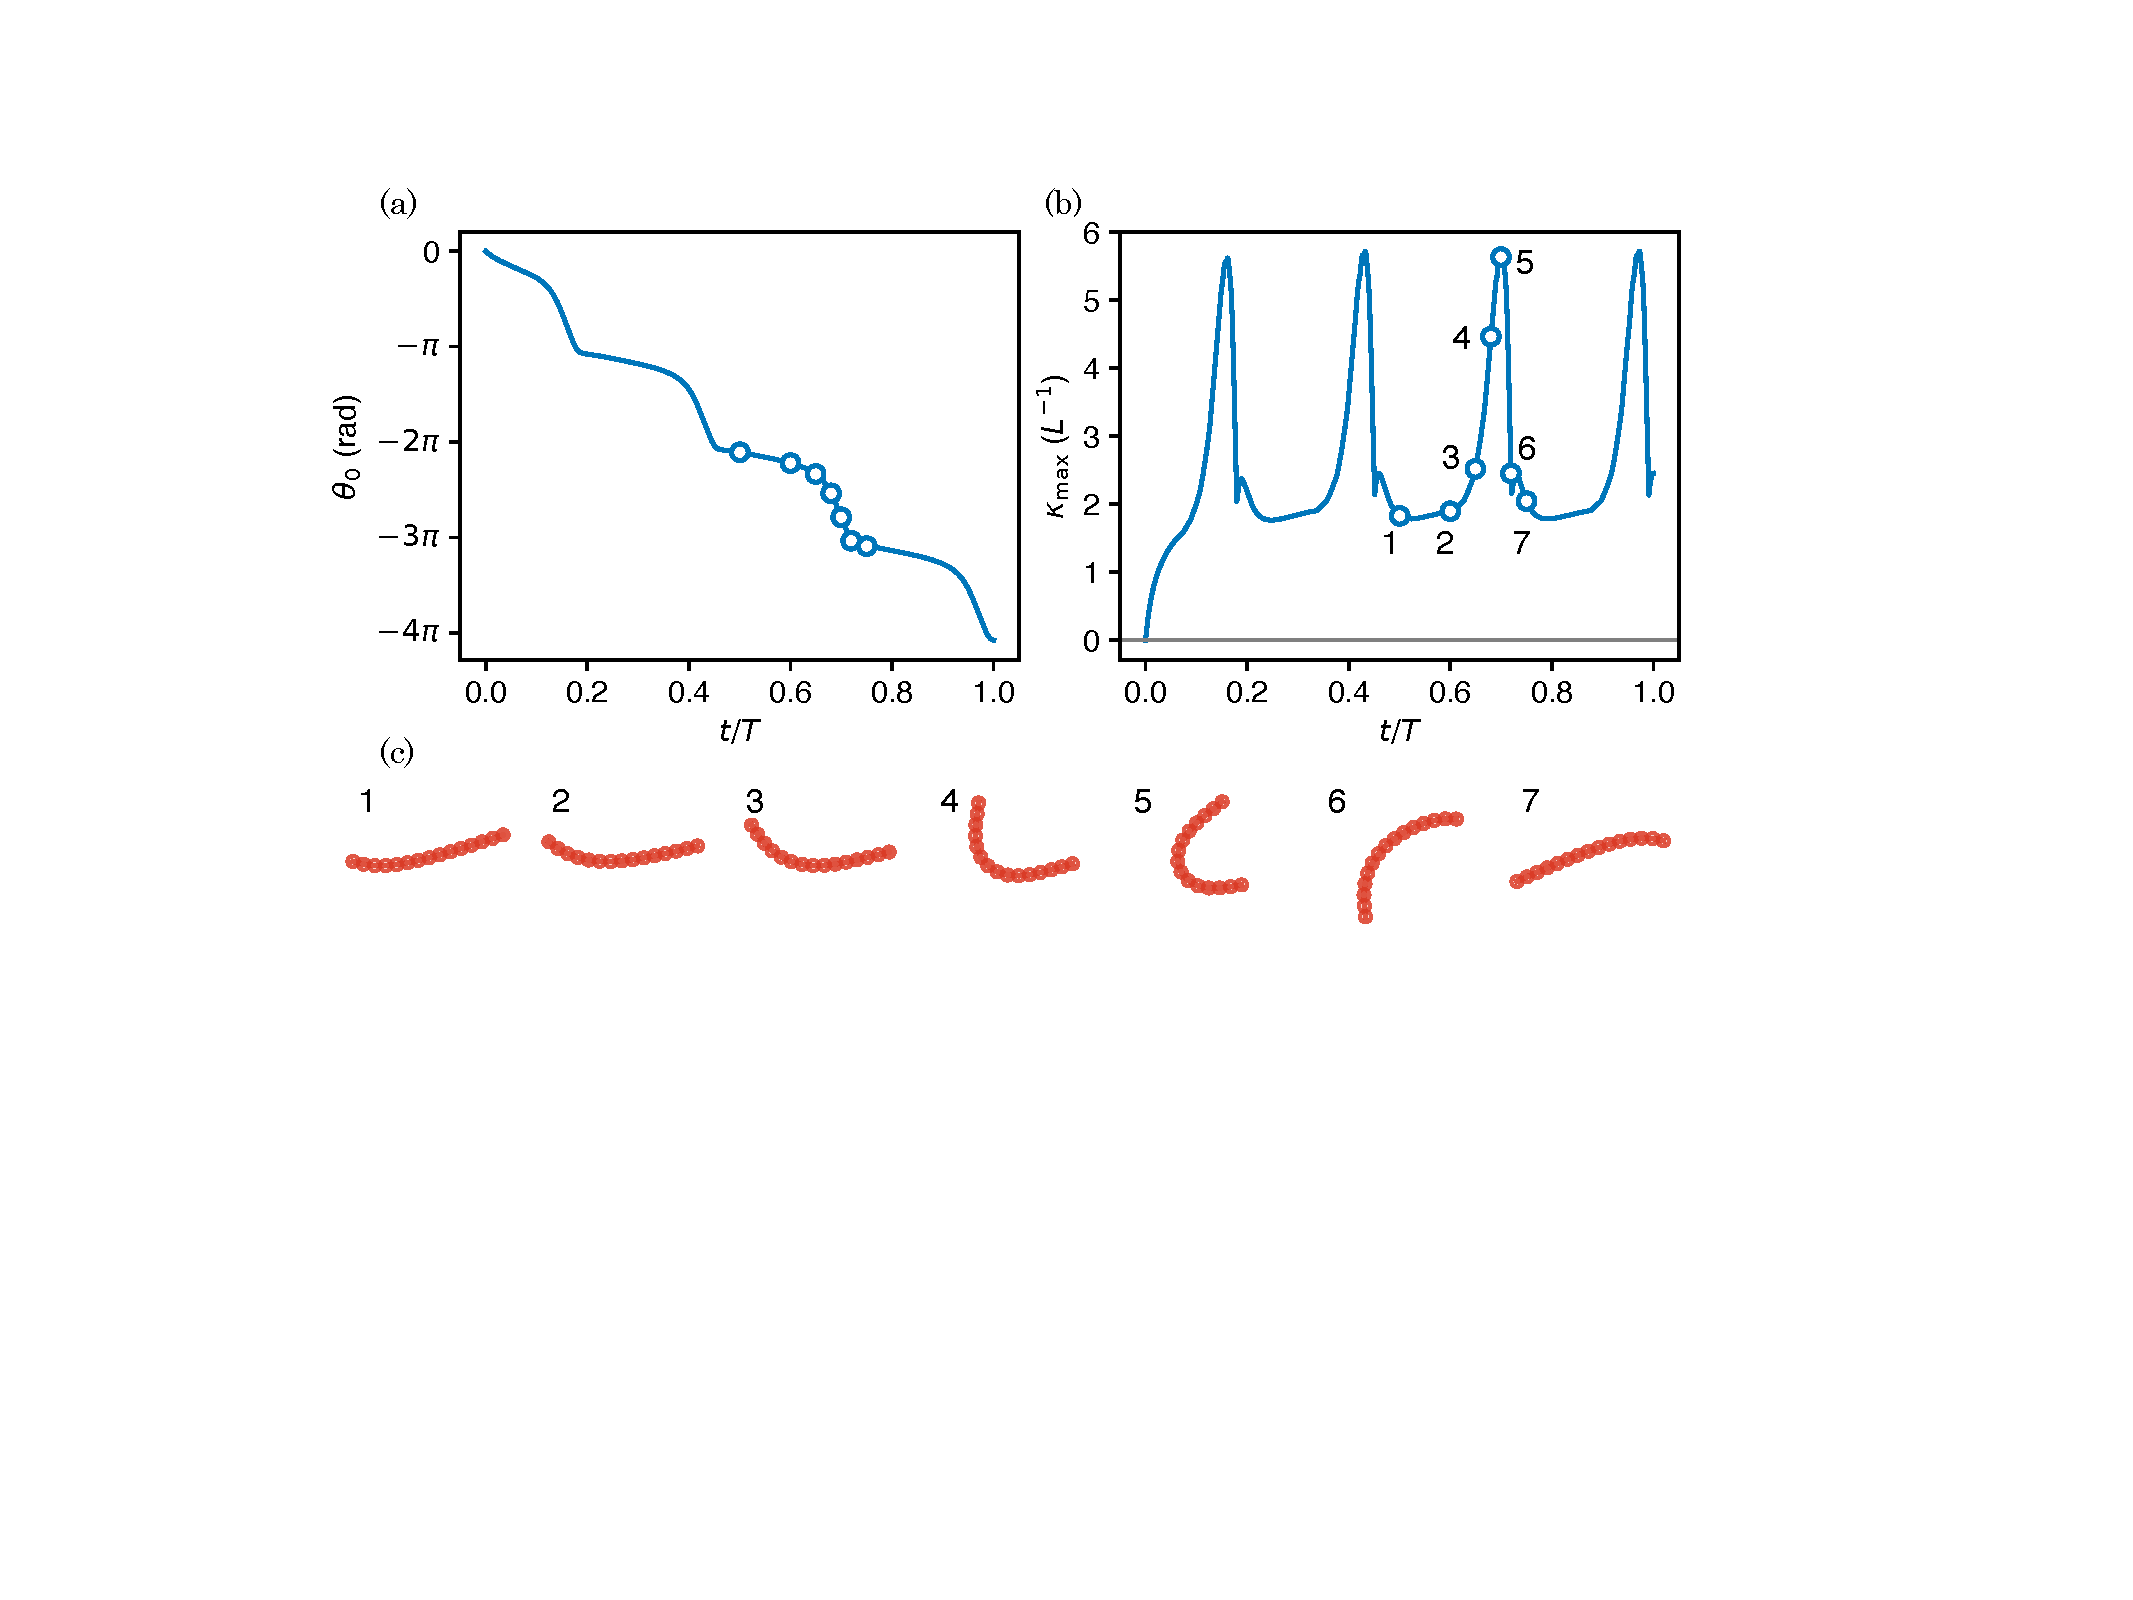
\includegraphics[scale=0.60]{./Figures/Fig7}
\caption{
	Flexible fiber tumbling in pure shear flow for a dimensionless bending rigidity $\bar B = B / (8\pi\mu\dot\gamma a^4)=200$. 
	(a) Orientation angle $\theta_0$ around $\be_3$ of the leftmost sphere as a function of time, normalised by the Jeffery's period of the rigid assembly $T$.
	(b) Maximum curvature of the fiber in units of length as a function of time. The horizontal grey line shows the intrinsic curvature of the fiber $\kappa_0 = 0.01 / L$.
	(c) Snapshots of the fiber deformation as labelled in (b).  
}
\label{fig:tumbling_fiber}
\end{center}
\end{figure}
%%%%%%%%%%%%%%%%%

Together, these three cases allow us to validate the numerical implementation of the soft degrees of freedom, the clamped boundary condition, and the coupling with the flow, in particular with the rate-of-strain tensor through $\tC_E$.

%%%%%%%%%%%%%%%%%%%%%%%%%%%%%%%%%%%%%%
\subsection{Jeffery's orbits}

We now place a rigid dumbbell made of two identical spheres in a pure shear flow. 
This axissymmetric body follows periodic trajectories, known as Jeffery's orbits~\cite{Jeffery1922, Bretherton1962, Thorp2019, Ishimoto2023}. 
The period and shape of the orbits are set by a single shape parameter $\beta$. 
For an ellipsoid of aspect ratio $c=a_\parallel / a_\perp$, the shape parameter is $\beta = (c^2 - 1) / (c^2 + 1)$. 
It was later generalised by Bretherton~\cite{Bretherton1962} to arbitrary axisymmetric bodies through an equivalent aspect ratio.
In our case, the Bretherton parameter $\beta$ is the component of the tensor $\tC_E$ coupling the component $\bE_3$ of the angular velocity $\bomega_0$ to the component $\bE_1 \otimes \bE_2$ of the rate-of-strain tensor $\tE_0^\infty$. 

Noting $\bE_1$ the dumbbell's axis of symmetry, the rigid mobility equation reduces to
\begin{equation}
\bEd_1 = \bomega_0^\infty \times \bE_{1} +
	\beta\left(\tE_0^\infty\cdot\bE_{1} - (\bE_{1}\cdot\tE_0^\infty\cdot\bE_{1})\bE_{1}\right).
\end{equation}
In a shear flow $\bu^\infty = \dot\gamma\,y\,\be_1$, the angular velocity and rate-of-strain tensor reduce to $\bomega_0^\infty =- \dot\gamma\be_3/2 $ and $\tE_0^\infty = \dot\gamma(\be_1 \otimes \be_2 + \be_2 \otimes \be_1)/2$. 
In spherical coordinates, $\bE_{1} = (\sin\theta\cos\varphi,\sin\theta\sin\varphi,\cos\theta)$ and the Jeffery's orbit admits an analytical solution such that
\begin{equation}\label{eq:Jeffery_solution}
\tan\varphi(t) = -\frac{1}{c} \tan\left(\frac{\dot\gamma t}{c+1/c} + \varphi_0 \right), \quad
\tan^2\theta \left(\cos^2\varphi + c^2\sin^2\varphi \right)=K^2,
\end{equation}
with  equivalent aspect ratio $c=\sqrt{(1+\beta)/(1-\beta)}$, period $T=2\pi(c+1/c)/\dot\gamma$, and
 constant of motion $K$, which is set by the initial condition.  
The above solution is now used to test the Python library implementation of the body-flow coupling.

The rigid body geometry is shown in Fig.~\ref{fig:Jeffery_rigid}a: it is made of two spheres of radius $a=1$ separated by a gap $\delta = 1$. 
The dumbbell's Bretherton parameter $\beta=0.717$ is recovered from the rigid mobility tensor and substituted into the analytical orbit.
In Figure~\ref{fig:Jeffery_rigid}, we compare the orbits computed from the library to the analytical solution given by Eq.~(\ref{eq:Jeffery_solution}), which agree within numerical precision. 


%%%%%%%%%%%%%%%%%
\begin{figure}[t]
\begin{center}
    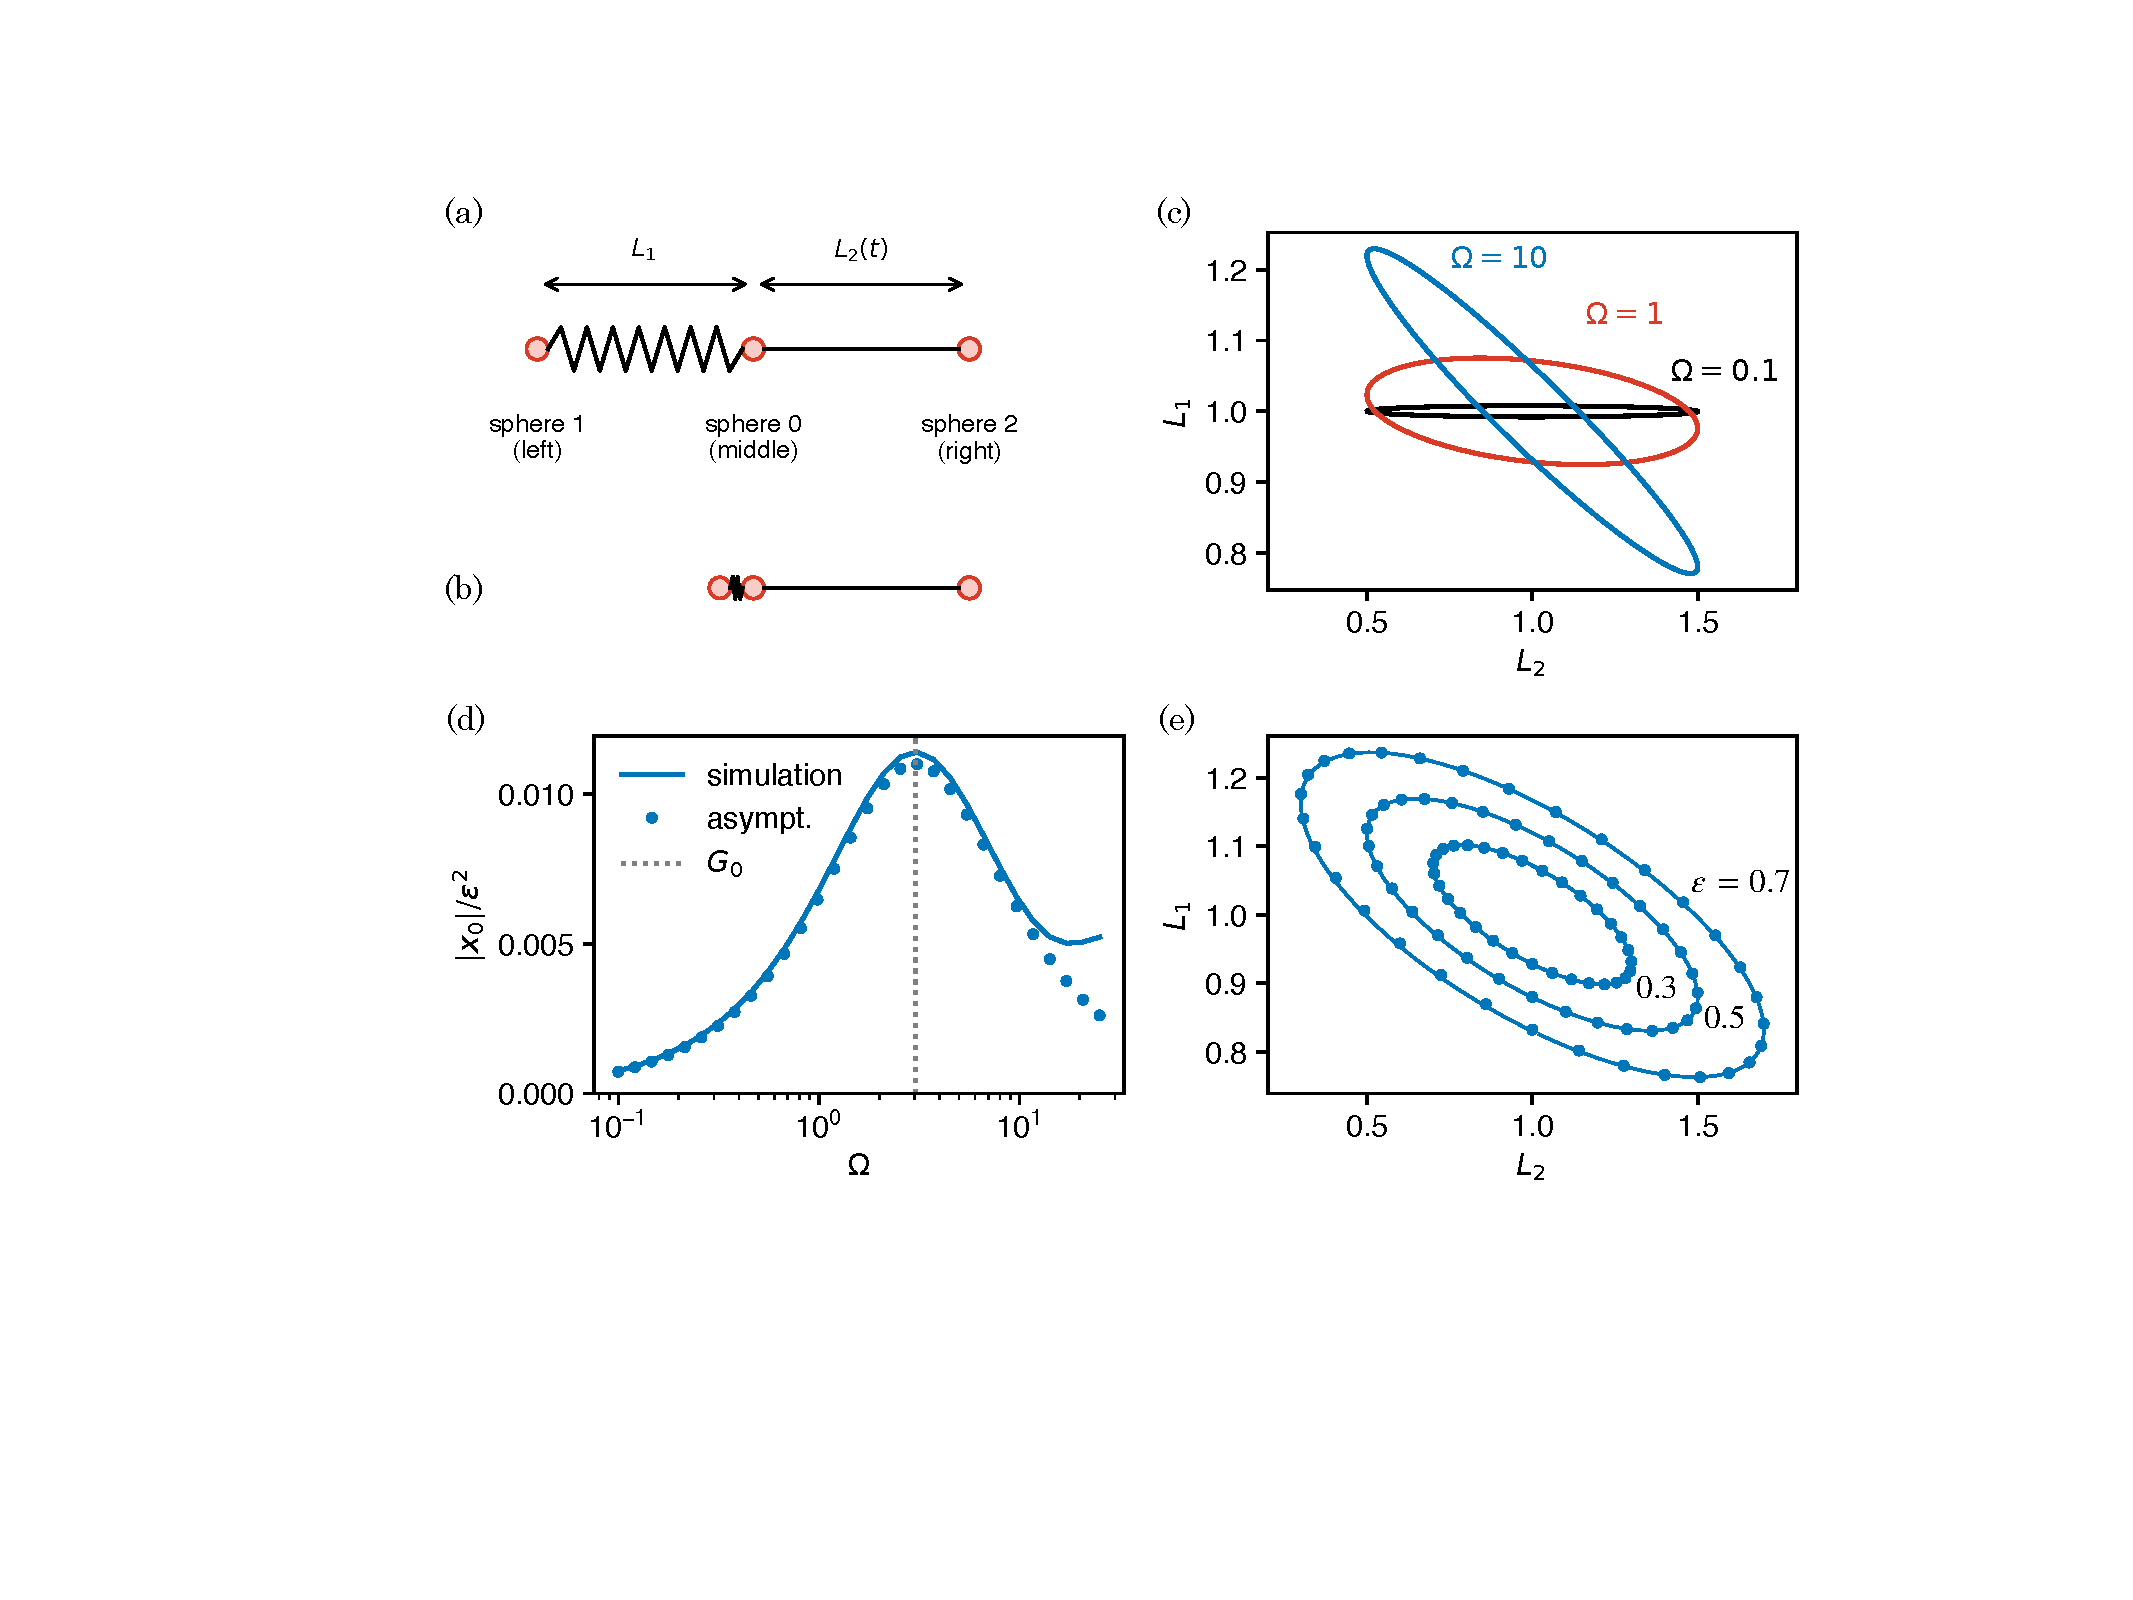
\includegraphics[scale=0.60]{./Figures/Fig8}
\caption{
	Jeffery orbits of a rigid dumbbell in a pure shear flow of unit shear rate in the $\be_1$-$\be_2$ plane: $\bu^\infty = [y, 0, 0]$.
	(a) Geometry of the rigid body considered in the body's frame.
	(b) Jeffery periodic orbits of $\bE_1$ in the laboratory's frame for different initial conditions (lines: simulation, dots: analytical solution).
	(c) Example of an orbit of $\bE_1$ as a function of time in the spherical coordinate $(r, \theta, \varphi)$.	
}
\label{fig:Jeffery_rigid}
\end{center}
\end{figure}
%%%%%%%%%%%%%%%%%


% Soft
Jeffery's orbits are degenerated, but the degeneracy can be lifted by a small amount of inertia, or a non-Newtonian rheology~\cite{Ishimoto2023}.
Another way to lift degeneracy is to add flexibility~\cite{Zhang2019}. This can be easily tested in the proposed library by replacing the rigid bond between the two spheres of the dumbbell by a linear spring of stiffness $k=100\mu \dot\gamma a$.
In that case, the orbits migrate towards the shear plane, as shown in Fig.~\ref{fig:jeffery_soft}.



%%%%%%%%%%%%%%%%%
\begin{figure}[bht]
\begin{center}
    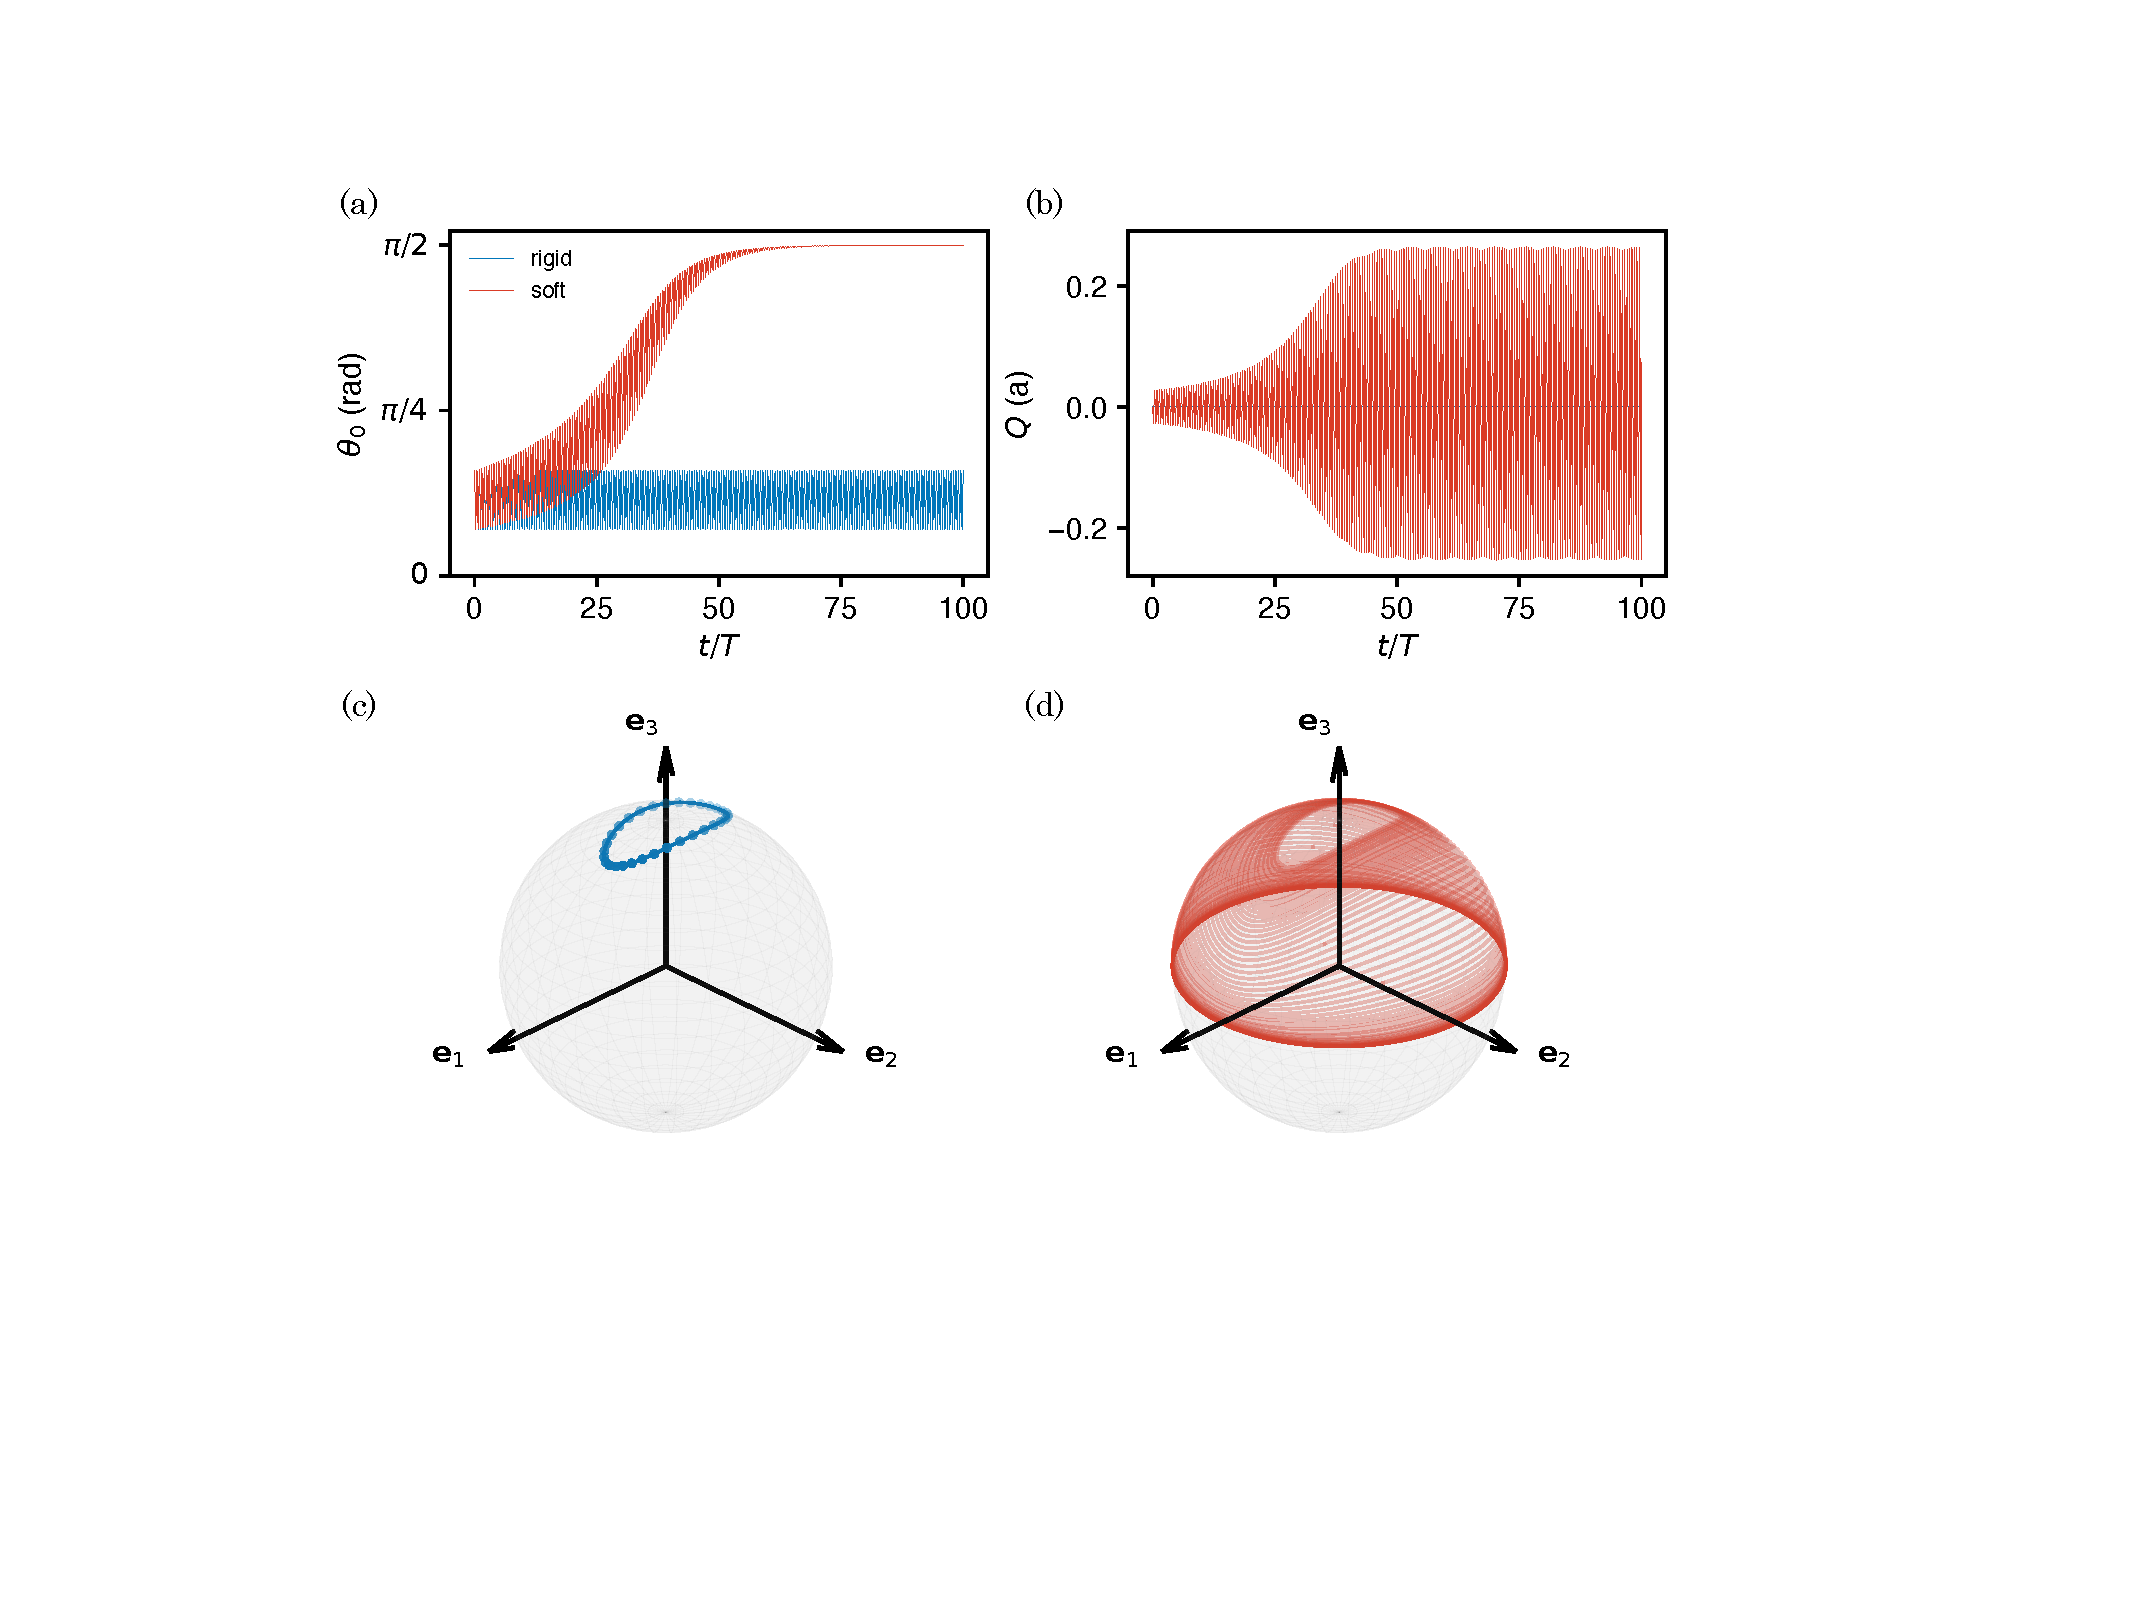
\includegraphics[scale=0.60]{./Figures/Fig9}
\caption{
	Jeffery's orbits of a soft dumbbell. 
	(a) Polar angle as a function of time for a rigid ($k=\infty$) and a soft ($k=100\mu \dot\gamma a$) dumbbell.
	(b) Elongation of the spring $Q$ in units of the sphere radius $a$. 
	(c) Similar to Fig.~\ref{fig:Jeffery_rigid} for the initial condition of (a). 
	(d) Orbit of $\bE_1$ the dumbbell's axis of symmetry, showing that the orbit is attracted to the shear plane $\be_1$--$\be_2$, corresponding to a polar angle $\theta=\pi /2$.
	}
\label{fig:jeffery_soft}
\end{center}
\end{figure}
%%%%%%%%%%%%%%%%%


%%%%%%%%%%%%%%%%%%%%%%%%%%%%%%%%%%%%%%
\subsection{Three-sphere swimmer}


We next turn to active swimming and optimization. 
Najafi and Golestanian proposed a simple three-sphere swimmer~\cite{Najafi2004}, which we use here for validation. 
This swimmer is made of three spheres of radii $a_i$ connected by deformable links, breaking time-reversal symmetry through a non-reciprocal actuation cycle (Fig.~\ref{fig:three_sphere}a). 
Here we drive the swimmer by a sinusoidal elongation $L_2 = l_2(1+\varepsilon\sin(\omega t))$ between the right and middle spheres. The left sphere is connected to the middle sphere by a passive spring of stiffness $k$ and rest length $l_1$. 
The problem is entirely determined by the dimensionless parameters
\begin{equation}
\Omega = \omega \mu (l_1 + l_2) / k, \quad
\varepsilon, \quad
l_1/l_2, \quad
a_i/l_2. 
\end{equation}

The goal is to find the rigidity, or equivalently $\Omega$, such that the displacement $x_0$ of the middle sphere over one period (after a transient) is maximum. Montino \& DeSimone~\cite{Montino2015} showed that the system admits a well-defined optimum $\Omega^* = G_0$ in the asymptotic limit of small $\varepsilon$, for fixed $\l_1/l_2$ and $a_i / l_2$. 
We will use their prediction as a benchmark of our optimization method. 

We set $\omega=l_2=\mu=1$ in the simulation and start with spheres of identical radii $a_i=0.05$ and $l_1=l_2$ (Fig.~\ref{fig:three_sphere}a). Varying the spring stiffness $k$ varies the dimensionless frequency $\Omega$. In  Fig.~\ref{fig:three_sphere}c, we show the periodic shape changes in the $L_1$--$L_2$ plane after a transient of four periods. For an optimal $\Omega^* = G_0$, the displacement over one period is maximized (Fig.~\ref{fig:three_sphere}d). We test that our numerical optimization predicts $G_0$ within less than 1\% for $\varepsilon=0.1$. Figure~\ref{fig:three_sphere}e shows that the simulation at this value of $\Omega$ reproduces the asymptotic predictions valid for small $\varepsilon$~\cite{Montino2015}.

To test the optimization method further, we optimize three design parameters: $k$, $a_1$, and $l_1$ (for fixed $a_0=a_2=0.05$, and $\varepsilon=0.5 l_2$). We show that the final shape (Fig.~\ref{fig:three_sphere}b) is $7.48$ times more efficient than the shape with $a_1=0.05$ and $l_1=1$ (optimal values: $k^*=1.19$, $a_1^*=0.049$, $l_1^*=0.155$). 


%%%%%%%%%%%%%%%%%
\begin{figure}[t]
\begin{center}
    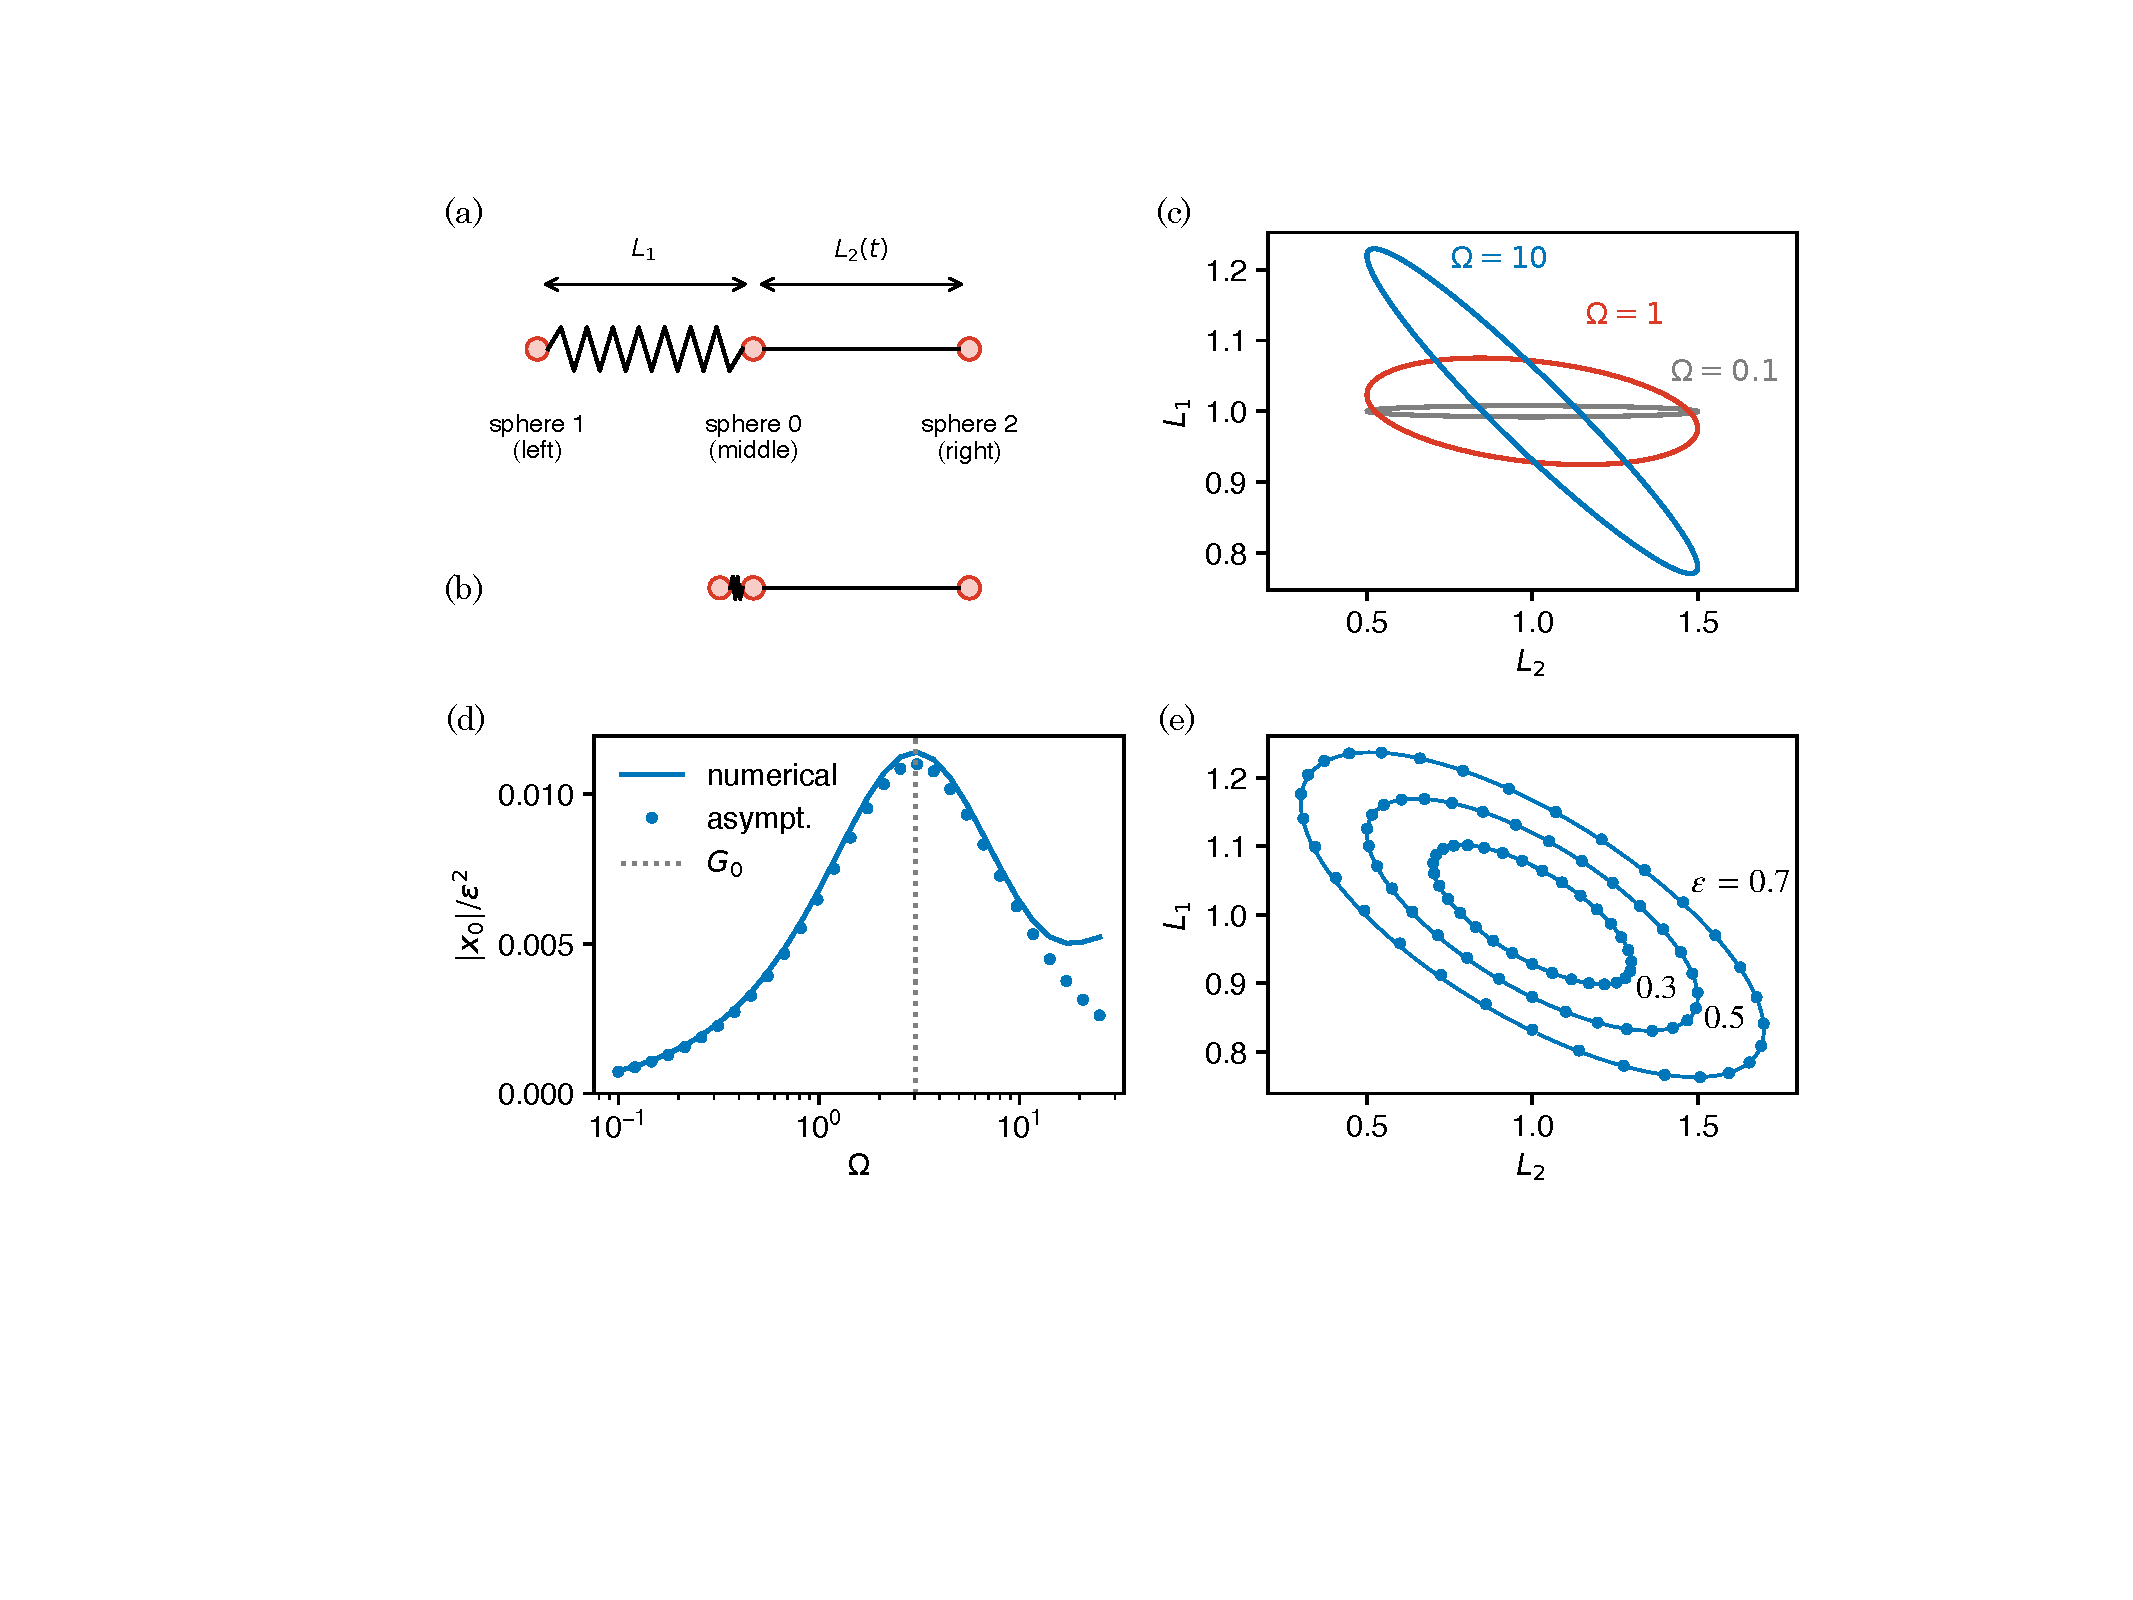
\includegraphics[scale=0.60]{./Figures/Fig10}
\caption{
	Optimization of the three-sphere swimmer.
	(a) Default geometry with $L_2 = 1+\varepsilon\sin(t)$, spring rest length $l_1=1$, and sphere radius $a_i=0.05$.
	(b) Optimized geometry for free $k$, $a_1$ and $l_1$.
	(c) Orbits of the swimmer in the $L_2$-$L_1$ plane for different values of the dimensionless frequency $\Omega = 2 / k$, with $k$ the spring stiffness. 
	(d) Swimming displacement over one period $|x_0|$ as a function of $\Omega$, for the default geometry and $\varepsilon = 0.1$ (line: simulation, dots: analytical asymptotics in the limit of small $\varepsilon$).
	(e) Orbits of the swimmer at optimal frequency $\Omega = G_0$ for different values of the forcing amplitude $\varepsilon$, as labelled. 
}
\label{fig:three_sphere}
\end{center}
\end{figure}
%%%%%%%%%%%%%%%%%




%%%%%%%%%%%%%%%%%%%%%%%%%%%%%%%%%%%%%%
\subsection{Soft surfer\label{sec.surfer}}

We now consider the optimization of a navigation problem: a gyrotactic swimmer in a Taylor--Green  flow~\cite{Colabrese2017}.
We will examine whether elastic deformations may help the swimmer to orient in the flow to ascend more rapidly passively.
The flow velocity of the Taylor--Green vortices is $\bu^\infty = V_\mathrm{max} [0, \sin(y/L)\cos(z/L), -\cos(y/L)\sin(z/L)]$, with typical length $L$, such that the maximum angular flow velocity is $\omega_\mathrm{max}=V_\mathrm{max}/L$.

We first consider a rigid bottom-heavy swimmer made of a light sphere, numbered 0, of radius $a_0$ and equivalent mass $m_0=-1$, and a heavy sphere of radius $a_1\leq a_0$ and opposite mass $m_1=1$ (Fig.~\ref{fig:surfers}a).
The swimming direction $\bE_3$ of this rigid swimmer follows the Pedley--Kessler equation \cite{Pedley1992}
\begin{equation}\label{eq:Pedley-Kessler}
\bEd_{3} = \bomega_0^\infty \times \bE_{3} + \beta\left(\tE_0^\infty\cdot\bE_{3} - (\bE_{3}\cdot\tE_0^\infty\cdot\bE_{3})\bE_{3}\right) + \frac{1}{2 \tau_\mathrm{align}} \left(\be_3 - (\be_3\cdot\bE_{3} ) \bE_{3}\right),
\end{equation}
where the first two terms on the right-hand side are due to the viscous torques and the third term to the gravitational torque.
In practice, for a rigid body with axis of symmetry $\bE_3$, the alignment timescale is $\tau_\mathrm{align} = 1/(2 m_1 g M_H)$, where $M_H$ is the entry of the mobility tensor $\tM_H$ that couples the $\bE_1$ component of the angular velocity $\bomega_0$ to the $\bE_2$ component of the gravitational force.
For the rigid body represented in Fig.~\ref{fig:surfers}a, we find $\tau_\mathrm{align} = 0.075 / \omega_\mathrm{max}$ for $m_1 g = 50 \mu a_0^2 \omega_\mathrm{max}$.

We integrate the mobility equation~(\ref{eq:soft_mobility_body}) for this bottom-heavy rigid swimmer by adjusting the active force such that the swimming velocity in a fluid at rest is $V_\mathrm{swim} = V_\mathrm{max}$. This is equivalent to integrating Eq.~(\ref{eq:Pedley-Kessler}) for the orientation, together with the equation $\bu_0 = \bu_0^\infty + V_\mathrm{swim}\bE_{3}$ for the translation. The trajectories for different initial positions are depicted in Fig.~\ref{fig:surfers}d. The swimmer tends to orient upwards, thanks to its bottom-heaviness, when it is near a separatrix where the vorticity is small. Otherwise, it tends to orient at an angle that can be obtained by balancing the viscous and gravitational torques in Eq.~(\ref{eq:Pedley-Kessler}). This equilibrium direction is illustrated in Fig.~\ref{fig:surfers}a for a steady vortical flow. It tends to move the swimmer in regions of smaller vertical velocity, which results in a preferential sampling of negative vertical flow velocities. This slows down the vertical migration and the effective vertical speed is $V_\mathrm{eff} = 0.567 V_\mathrm{swim}$ for the 15 initial conditions tested in Fig.~\ref{fig:surfers}d and a simulation time of $T=4\pi/ \omega_\mathrm{max}$. In other words, the vertical translation is slowed down by the background flow for a rigid gyrotactic swimmer. 

%%%%%%%%%%%%%%%%%
\begin{figure}[t]
\begin{center}
    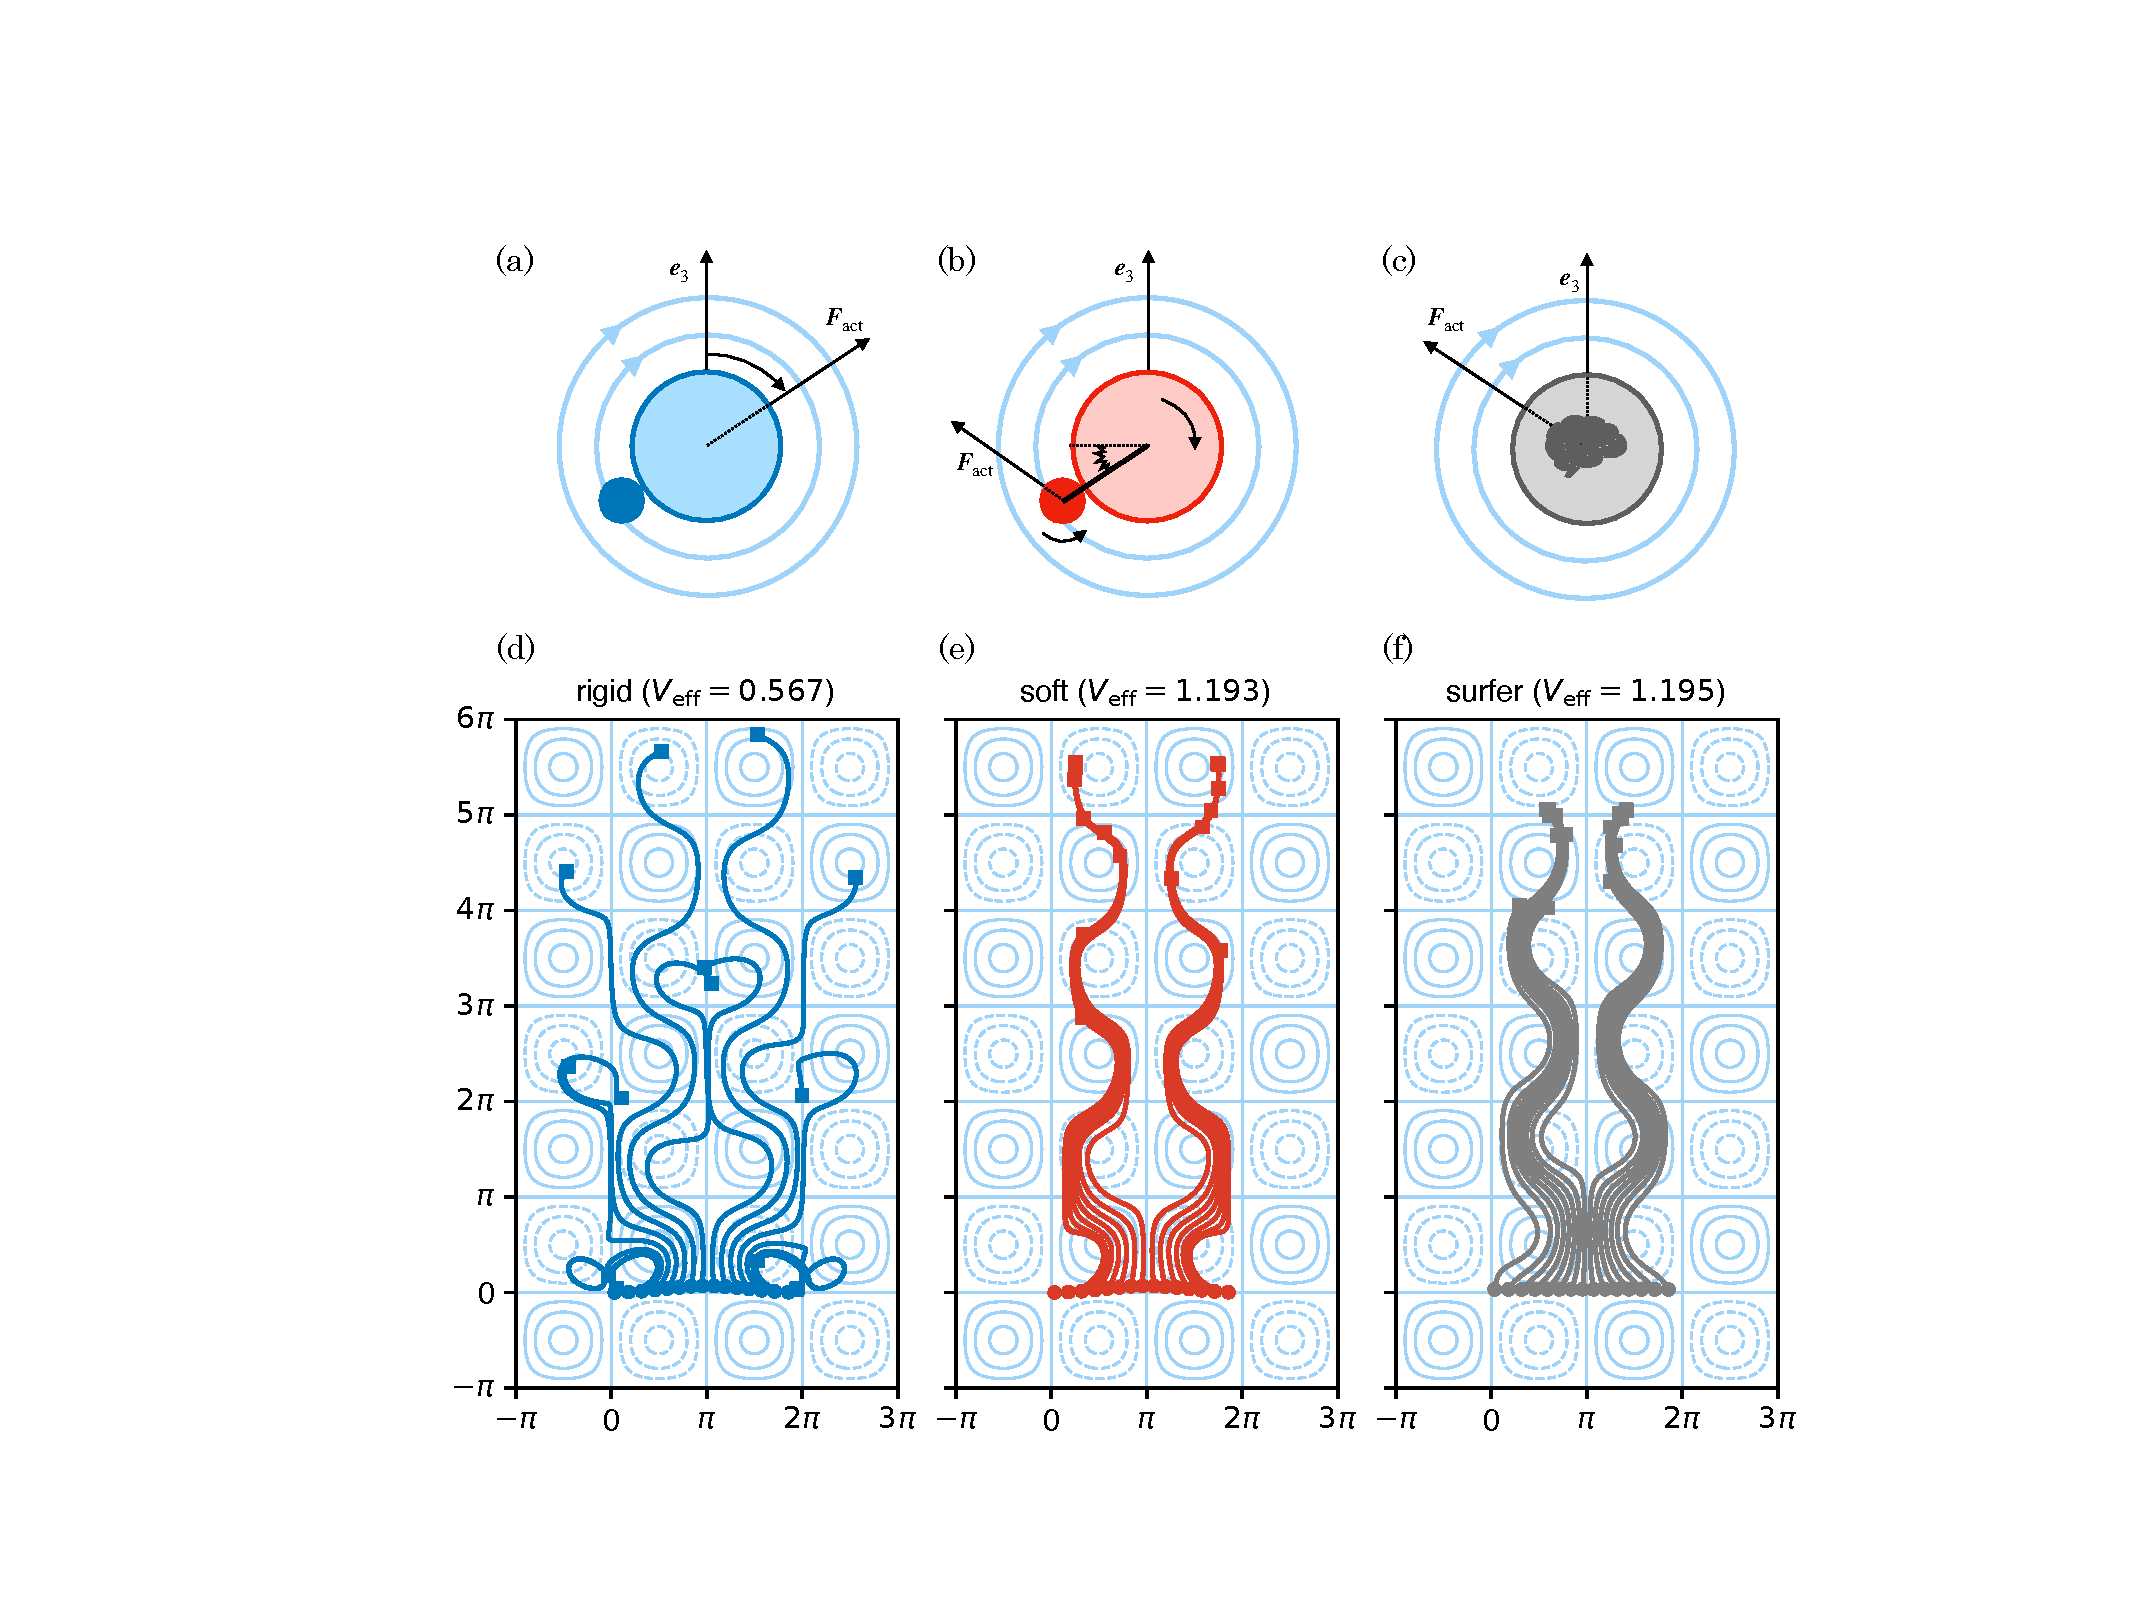
\includegraphics[scale=0.60]{./Figures/Fig11}
\caption{
	Vertical migration by gyrotactic swimmers in a flow.
	We consider three types of swimmers:
	(a) a rigid asymmetric dumbbell with the small sphere heavier than the large one;
	(b) a soft swimmer with the same shape as (a) but with the two spheres able to roll on each other, with a torsional pull-back spring;
	(c) a surfer, which chooses the direction of swimming according to the surfing policy aligned with $\be_3\cdot \exp(\tau \nabla \bu^\infty)$.
	These three swimmers with identical swimming speed $V_\mathrm{swim}$ have different trajectories in a Taylor--Green vortical flow:
	(d) rigid swimmers can get trapped in vortical cells and their effective vertical velocity is $V_\mathrm{eff} = 0.567 V_\mathrm{swim}$; 
	(e) soft swimmers ``slalom'' the vortical cells and enhance their effective vertical velocity to $V_\mathrm{eff} = 1.193 V_\mathrm{swim}$;
	(f) surfers reach a similar effective vertical velocity of $V_\mathrm{eff} = 1.195 V_\mathrm{swim}$ with a more conservative strategy (more vertical).
	Light blue lines represent the flow streamlines (dashed for negative vorticity, solid for positive vorticity). 
	}
\label{fig:surfers}
\end{center}
\end{figure}
%%%%%%%%%%%%%%%%%

We now consider the same geometry, but instead of having a rigid body, the two spheres are able to roll onto each other with a torsional spring of stiffness $k$ (Fig.~\ref{fig:surfers}b). The active force producing the swimming is now attached to the heavy sphere, such that it is not necessarily aligned with $\bE_3$: $\bE_3$ remains aligned with the axis joining the centers of the two spheres, but the orientation of each sphere is different with orientation vectors satisfying $a_1 \btheta_1 = -a_0\btheta_0$ (condition for rolling without slip).
Flexibility adds a dimensionless rigidity to the problem: $\bar k = k/(\mu \omega_\mathrm{max} a_0^3)$.
Through the optimization, we found the design parameters of this soft swimmer that maximize the average effective vertical velocity $V_\mathrm{eff}$ for the same 15 initial conditions as the rigid gyrotactic swimmer and the same simulation time of $T=4\pi/ \omega_\mathrm{max}$.
These optimal parameters are $a_1/a_0=0.169$ and $\bar k = 18.2$, and the effective velocity is $V_\mathrm{eff} = 1.193 V_\mathrm{swim}$, which means that this soft swimmer swims 19\% faster than without background flow (Fig.~\ref{fig:surfers}e).

The mechanism behind this speed-up is the following. In a quiescent fluid, the torsional spring relaxes both sphere orientations to zero, the swimming direction then coincides with the bottom-heavy axis $\bE_3$, and the soft swimmer behaves like the rigid one. In a vortical flow, the viscous torques on the two spheres have opposite signs, but the light sphere being larger, its torque is larger in absolute value. Together with the rolling constraint $a_1\btheta_1 = -a_0\btheta_0$ and the spring restoring force, the torques set an equilibrium with a small angular offset between the heavy sphere and $\bE_3$, whose amplitude is controlled by $a_1/a_0$ and $\bar k$. Two limits frame the design space: for stiff springs ($\bar k \to \infty$) the offset vanishes and the soft swimmer recovers the rigid one; for floppy springs ($\bar k \to 0$) the swimming direction decouples from $\bE_3$ entirely, so that gravity loses its ability to reorient the swimmer. The optimum $(a_1/a_0, \bar k) = (0.169, 18.2)$ found by the optimization lies in between, where the offset is just large enough to tilt the swimming axis in the opposite sense to that of the rigid swimmer: a mirror swimming direction with the same bottom-heavy axis (Fig.~\ref{fig:surfers}b). The bottom-heavy axis still points toward regions of negative vertical flow, but the swimming axis now points toward regions of positive vertical flow. This reversal of the gyrotactic bias produces the preferential sampling of upward flow and the 19\% speed-up of $V_\mathrm{eff}$ over $V_\mathrm{swim}$.


We compare this performance with that of a surfer that chooses its swimming direction according to the surfing strategy of Ref. \cite{Monthiller2022}, which aligns the swimming direction along $\be_3\cdot\exp(\tau\nabla\bu^\infty)$ with a time delay $\tau_\mathrm{align}$ to make a fair comparison with the rigid or soft gyrotactic swimmers considered before. 
This surfing strategy is based on a linear approximation of the background flow integrated during a typical correlation time $\tau$. We have shown that this strategy is quasi-optimal for turbulent flows~\cite{Mecanna2025}.
Here $\tau$ can be viewed as a parameter that has to be optimized for maximal $V_\mathrm{eff}$: we find $\tau = 0.547 / \omega_\mathrm{max}$ and $V_\mathrm{eff}= 1.195 V_\mathrm{swim}$. So the performance is identical to that of the optimal soft swimmer, with trajectories that are slightly more vertical  (Fig.~\ref{fig:surfers}f).

%%%%%%%%%%%%%%%%%%%%%%%%%%%%%%%%%%%%%%%%%%%%%%%%%%%%%%%%%%%%%%%%%%%%%%%%%%%%%
\section{Discussion\label{sec.discussion}}

%Summary
We have presented a soft mobility framework that extends classical rigid-body mobility theory to deformable bodies in Stokes flow. Starting from the continuum elastohydrodynamic problem of a hyperelastic body in a linearized background flow, the principle of virtual power and the Lorentz reciprocal theorem yield a weak formulation [Eq.~(\ref{eq:weak_form})] amenable to Galerkin discretization. Specializing to assemblies of rigid spheres connected by springs gives a closed-form, configuration-dependent ordinary differential equation~(\ref{eq:soft_mobility_body}), in which the soft mobility tensors are explicit functions of the deformation state. The framework was validated on canonical problems and exploited as an inverse-design tool through end-to-end automatic differentiation, illustrated by the soft surfer: a passive gyrotactic swimmer whose flexibility turns a slowdown into a speedup.


%Relation to existing frameworks
The soft mobility equation~(\ref{eq:soft_mobility_body}) sits between two established families. Bead and multiblob methods \cite{Delmotte2015,Balboa-Usabiaga2022,Fuchter2023} discretize a deformable body into rigid sub-bodies and enforce inter-bead constraints by solving a saddle-point linear system at every timestep. This is efficient for forward simulation, but the implicit constraint solve is costly to differentiate, which makes shape optimization difficult. At the other end, the generalized-coordinate framework of Solovev and Friedrich \cite{Solovev2021} projects the deformation onto a small set of Lagrangian coordinates and balances generalized forces in the space of generalized coordinates. Their formulation is closest in spirit to ours, but it is designed for active microswimmers (tabulated hydrodynamic forces, no coupling to a background flow, no elastic energy term) and is not constructed for differentiability.

The present framework combines the projection idea of Ref.~\cite{Solovev2021} with three additions: a closed-form differentiable mobility (here Rotne--Prager--Yamakawa, though any differentiable mobility model is compatible), explicit elastic and flow-coupling tensors, and a JAX implementation that makes every tensor differentiable with respect to the design parameters. The cost of one forward simulation exceeds that of an explicit bead-spring or multiblob simulation, but the gradient of any scalar objective with respect to the design parameters comes essentially for free through reverse-mode automatic differentiation.

%Scope and cost
The soft mobility theory is tailored for systems with few degrees of freedom, typically $N_Q = \mathcal{O}(1)$, in contrast with standard Stokesian dynamics approaches that handle suspensions with $N_Q = \mathcal{O}(N)$, where $N = \mathcal{O}(10^3)$ rigid bodies or more~\cite{Brady1988,Fiore2019,Swan2016}. Those methods invert the saddle-point system arising from the constraints using preconditioned iterative solvers (typically GMRES~\cite{Saad1986}, with $\mathcal{O}(N^2)$ scaling per timestep, or $\mathcal{O}(N)$ when combined with fast multipole methods~\cite{Greengard1987,Tornberg2008,Liang2013}).
These iterative procedures are efficient for forward simulation but difficult to differentiate by reverse mode, because storing the intermediate states of the iterative solver incurs a prohibitive memory cost. Our framework instead inverts the dense $6N\times 6N$ grand mobility matrix directly in Eq.~(\ref{eq:projection}). This $\mathcal{O}(N^3)$ inversion is computationally costly, but it is differentiable. For small $N_Q$, the inversion can be tabulated on a discrete grid in $\bQ$ and interpolated during simulation, making the cost competitive with iterative approaches. The framework is therefore most useful when one wants to optimize the design of a single deformable body, and least competitive when one wants to simulate large suspensions for which Stokesian dynamics remains the right tool.

%Modeling assumptions
Beyond this scope question, two modeling assumptions bound the domain of validity. The background flow is linearized around the body, which assumes $L \ll \eta$, where $L$ is the body size and $\eta$ the smallest scale of the flow. The Rotne--Prager--Yamakawa approximation is a pairwise far-field expansion that breaks down at lubrication contact between spheres; problems with nearly touching elements would require lubrication corrections~\cite{Brady1988,Fiore2019} or a different mobility model, which the framework accommodates as long as that model remains differentiable.

%Future avenues
Soft mobility theory could be extended in three directions. First, Brownian fluctuations could be added by including a stochastic force term in the soft mobility equation, calibrated to satisfy the fluctuation--dissipation theorem on the reduced generalized coordinates. This would extend the framework to soft macromolecules and microswimmers in thermal baths, and connect it to recent work on Brownian dynamics \cite{Cichocki2021,Funkenbusch2024}. 
%2
Second, far-field hydrodynamic interactions between soft bodies could be incorporated by treating each soft body as a deformable multipole and coupling them through the RPY tensor (or a truncated Fax\'en expansion) evaluated at the inter-body separations. Pairs and dilute suspensions of soft bodies in flow would then become tractable, opening the soft-mobility analogue of Stokesian dynamics for dilute suspensions of deformable bodies, complementing existing Stokesian dynamics for rigid suspensions \cite{Brady1988,Fiore2019}.
%3
Finally, the differentiable rollout invites systematic inverse-design campaigns: optimizing flexible microswimmers for magnetic actuation or for navigation in turbulent flows, designing passive shapes for clustering, sorting, or escape, and learning soft-body controllers in the spirit of morphological computation~\cite{Pfeifer2014,Hauser2014} and physical intelligence~\cite{Sitti2021}. The soft surfer of \S\ref{sec.surfer} is a first proof of concept in this direction.


%%%%%%%%%%%%%%%%%%%%%%%
\begin{acknowledgments}
Most of this work has been developed during a sabbatical stay in Cambridge, funded by the French Embassy Churchill College Fellowship.
This project has received funding from the European Research Council (ERC) under the European Union’s Horizon 2020 research and innovation program (grant agreement No 834238).
\end{acknowledgments}


\appendix

%%%%%%%%%%%%%%%%%%%%%%%%%%%%%%%%%%%%%%%%%%%%%%%%%%%%%%%%%%%%%%%%%%%%%%%%%%%%%
\section{Continuum mechanics}

%%%%%%%%%%%%%%%%
\subsection{Surface Jacobian}
The surface integral can also be expressed in the deformed configuration
\begin{equation}\label{eq:surface_integral}
\int_{\partial \Omega_0} \bF_s \cdot \bV^* \, \rmd S = 
	\int_{\partial \Omega_t} \bff_s \cdot \bV^* \, \rmd s =
	\int_{\partial \Omega_0} J_s \bff_s \cdot \bV^* \, \rmd S,
\end{equation}
with $\bff_s = \tsigma\cdot \bn$ the traction (in the deformed configuration), the force exerted by the fluid on the body,
where $\tsigma$ is the Cauchy stress tensor. We thus have $\bF_s= J_s \bff_s$ with $J_s$ the Jacobian of the surface deformation
\begin{equation}\label{eq:surface_Jacobian}
J_s= \|\tF^{-\top}\cdot \bN\| \det(\tF). 
\end{equation}

%%%%%%%%%%%%%%%%
\subsection{Boundary integral equation\label{sec:BIE}}
The hydrodynamic traction $\bff_s(\bz)$ at a point $\bz\in\partial\Omega_t$ is determined by the boundary integral formulation of the Stokes equations \cite{Pozrikidis1992}. By linearity, the surface traction and the surface velocity are related through
\begin{eqnarray}
\bu(\bz) & = & 
	- \frac{1}{4\pi\mu} \int_{\partial \Omega_t}
		\tG(\by - \bz)\cdot\bff_s(\by)\, \rmd s(\by) 
	+ \frac{1}{4\pi} \int_{\partial \Omega_t}
		\bu(\by) \cdot \bT(\by - \bz)\cdot\bn(\by)\, \rmd s(\by), \label{eq:boundary_integral_orig}\\
		& = & 
	- \frac{1}{8\pi\mu} \int_{\partial \Omega_t}
		\tG(\by - \bz)\cdot\bff_s(\by)\, \rmd s(\by) 
	+ \frac{1}{8\pi} \int_{\partial \Omega_t}
		\left[\bu(\by)-\bu(\bz)\right] \cdot \bT(\by - \bz)\cdot\bn(\by)\, \rmd s(\by),\label{eq:boundary_integral_nonsingular} 
\end{eqnarray}
with 
\begin{eqnarray}
\tG(\br) & = & \frac{\tI}{r}  + \frac{\br \otimes \br}{r^3},\\
\bT(\br) & = & - 6 \frac{\br \otimes \br  \otimes \br}{r^5},
\end{eqnarray}
where $\tG$ is the second-order stokeslet Oseen tensor, $\bT$, the corresponding third-order stress tensor, and $r=\|\br\|$. Both Eqs. (\ref{eq:boundary_integral_orig}) and (\ref{eq:boundary_integral_nonsingular}) are equivalent. In Eq. (\ref{eq:boundary_integral_nonsingular}), subtracting $\bu(\bz)$ from $\bu(\by)$ in the double-layer integrand cancels the $1/r^2$ singularity of $\bT$, so the integral is weakly singular and standard Gauss quadrature applies.

Setting $\bu(\bz) = \bV^*(\bz)$ on $\partial\Omega_t$ in Eq.~(\ref{eq:boundary_integral_nonsingular}) yields the virtual traction $\bff_s^*$ required in the reciprocal theorem (\ref{eq:reciprocity}).


%%%%%%%%%%%%%%%%%%%%%%%%%%%%%%%%%%%%%%
\subsection{Galerkin discretization\label{sec:Galerkin}}
Equation~(\ref{eq:weak_form}) is a weak formulation on infinite-dimensional space $V$. 
To obtain a finite-dimensional system, we restrict $\bxd$ to a subspace $V_n\subset V$ spanned by $n$ basis functions $\{\bV_j\}$ and write
\begin{equation}
\bxd (\bX,t) =  \sum_{j=1}^n \dot{a}_j(t)\, \bV_j(\bX).
\end{equation}
Testing Eq.~(\ref{eq:weak_form}) with each $\bV_i$ and using the linearity in $\bu_0^\infty$, $\bomega_0^\infty$, and $\tE_0^\infty$ yields the projected system
\begin{equation}\label{eq:galerkin_system}
\hat{\tR} \cdot \dot{\ba} + \hat{\tK}_{NL} - \hat{\tC}_H\cdot\bH + \hat{\tC}_V \cdot \bv_0^\infty + \hat{\tC}_E : \tE_0^\infty = 0,
\end{equation}
where $\ba = [a_1,\dots a_n]$, $\bv_0^\infty$ is the six-component flow velocity $[\bu_0^\infty,\bomega_0^\infty]$, and $\tE_0^\infty$ is rate-of-strain tensor, which in practice is represented as a 5-component vector (see Appendix~\ref{app:strain_vec}). All tensors depend on the current configuration $\bchi(\bX,t)$. The resistance matrix $\hat{\tR}$ is symmetric positive definite by virtue of the reciprocal theorem. The nonlinear stiffness $\hat{\tK}_{NL}$ is symmetric positive semi-definite by its relation to the elastic energy. Note that hatted tensors refer to the abstract Galerkin discretization. The same letters without a hat refer to their sphere-assembly realization below.

The general Galerkin framework described here applies to any compatible velocity basis $\{\bV_j\}$. For bodies composed of rigid spheres connected by elastic links, the natural choice is the rigid-body modes of each sphere. The sphere-assembly discretization developed in \S{sec.kinematics} is the specialization of the Galerkin method to this basis.


%%%%%%%%%%%%%%%%%%%%%%%%%%%%%%%%%%%%%%%%%%%%%%%%%%%%%%%%%%%%%%%%%%%%%%%%%%%%%
\section{Sphere assembly kinematics}

%%%%%%%%%%%%%%%
\subsection{Bortz equation\label{app:bortz}}

The orientation of a rigid body in three dimensions is parameterized by the Rodrigues vector $\bTheta\in\mathbb{R}^3$: its direction $\hTheta = \bTheta/\Theta$ (with $\Theta = \|\bTheta\|$) is the rotation axis and its magnitude $\Theta$ is the rotation angle. The corresponding rotation matrix is given by the Euler--Rodrigues formula
\begin{equation}\label{eq:Rodrigues_formula}
\mRot(\bTheta) = \cos\Theta\,\tI + \sin\Theta\,[\hTheta]_\times + (1-\cos\Theta)\,\hTheta\otimes\hTheta,
\end{equation}
with $\otimes$ the outer product.
Laboratory-frame coordinates $\bx$ and body-frame coordinates $\bX$ are related by $\bx = \mRot(\btheta_0)\cdot\bX$.
This parameterization is singularity-free for $\Theta\in[0,2\pi)$, unlike Euler angles, which suffer from gimbal lock.

A natural but incorrect assumption would be that the  velocity $\bOmega$ equals $\bThetad$. The correct relation follows from differentiating the Euler--Rodrigues formula with respect to time \cite{Bortz1971}\begin{equation}\label{eq.Bortz_kinematics}
\bOmega = \tB_3(\bTheta) \cdot \bThetad,
\end{equation}
with the $3\times 3$ Bortz matrix
\begin{equation}\label{eq.Bortz_one_sphere}
\tB_3(\bTheta) =
	\frac{\Theta}{2}\cotan\!\left(\frac{\Theta}{2}\right)\tI
	- \frac{\Theta}{2}\left[\hTheta\right]_\times
	+ \left(1 - \frac{\Theta}{2}\cotan\!\left(\frac{\Theta}{2}\right)\right)\hTheta\otimes\hTheta.
\end{equation}
In the limit $\Theta\to 0$, $\tB_3\to\tI$ (using $\frac{\Theta}{2}\cotan\frac{\Theta}{2}\to 1$), recovering the expected identity $\bOmega\to\bThetad$.

This relation is used to compute the six-component velocity $\bV_i$ of the $i$-th sphere from the time-derivative of its six-component position $\bX_i$ in \S\ref{sec.kinematics}.
The translational velocity of the sphere center follows directly from its position, $\bU_i = \bRd_i$. For the rotational part, $\bOmega_i = \tB_3(\bTheta_i) \cdot \bThetad_i$.
Stacking translation and rotation, the Bortz Jacobian for sphere $i$ is the $6\times 6$ block-diagonal matrix
\begin{equation}\label{eq:B6}
\tB_6(\bTheta_i) =
\begin{bmatrix} \tI & \mathbf{0} \\ \mathbf{0} & \tB_3(\bTheta_i) \end{bmatrix},
\quad\text{so that}\quad
\bV_i = [\bU_i, \bOmega_i] = \tB_6(\bTheta_i)\cdot[\bRd_i,\bThetad_i].
\end{equation}
The Bortz matrix $\tB$ used in the main text is a $(6+N_Q)\times(6+N_Q)$ matrix, whose upper-left block is $\tB_6(\btheta_0)$, the lower-right block is the identity $\tI$, the non diagonal blocks being $\bm{0}$. It is used to transform generalized coordinates $\bq$ into generalized velocities $\bp$, such that $\bp = \tB\cdot\bqd$. 

The Bortz matrix $\tB_3$ becomes singular as $\Theta\to 2\pi$, where $\cotan(\Theta/2)\to\pm\infty$. To keep the integration well-conditioned, the Rodrigues vector is remapped after each time step: whenever $\|\bTheta\|\geq\pi$,
\begin{equation}
\bTheta \;\leftarrow\; \bTheta - 2\pi\,\hTheta.
\end{equation}
This subtracts one full turn along the rotation axis. Since a rotation by $\Theta$ and a rotation by $\Theta - 2\pi$ about the same axis produce the same orientation, the physical state is unchanged. The remapping reduces the angle magnitude to $2\pi - \Theta \leq \pi$, keeping $\|\bTheta\|$ bounded away from the singularity at $2\pi$ throughout the simulation.

%%%%%%%%%%%%%%%
\subsection{Rate-of-strain vectorization\label{app:strain_vec}}

The rate-of-strain tensor $\tE_0^\infty$ is symmetric and traceless. Symmetry reduces its nine components to six independent entries, and the tracelessness condition $\mathrm{tr}(\tE_0^\infty) = 0$ removes one further degree of freedom, leaving five independent components. We parameterize them as the vector
\begin{equation}\label{eq:strain_vec}
\bE^\infty_\mathrm{vect} = [E_{11},\, E_{12},\, E_{13},\, E_{22},\, E_{23}],
\end{equation}
from which the full tensor is recovered as
\begin{equation}\label{eq:strain_mat}
\tE_0^\infty =
\begin{pmatrix}
E_{11} & E_{12} & E_{13} \\
E_{12} & E_{22} & E_{23} \\
E_{13} & E_{23} & -E_{11}-E_{22}
\end{pmatrix},
\end{equation}
with the $(3,3)$ entry $E_{33} = -E_{11}-E_{22}$ enforcing tracelessness.

The double contractions $\hat{\tC}_E:\tE_0^\infty$ and $\tC_E:\tE_0^\infty$ appearing in Eqs.~(\ref{eq:galerkin_system}) and (\ref{eq:soft_mobility}) can each be expressed as a matrix-vector product with $\bE^\infty_\mathrm{vect}$. Because every entry $(\tE_0^\infty)_{jk}$ is a linear combination of the five components $E_l$ [Eq.~(\ref{eq:strain_mat})], the double contraction
\begin{equation}
\left(\tC_E:\tE_0^\infty\right)_i = \sum_{j,k}(C_E)_{ijk}\,(\tE_0^\infty)_{jk}
\end{equation}
is linear in $\bE^\infty_\mathrm{vect}$, so it can be written as $\tC_E^{(5)}\cdot\bE^\infty_\mathrm{vect}$ for an equivalent $N_q\times 5$ matrix $\tC_E^{(5)}$. The entries of $\tC_E^{(5)}$ are obtained by substituting Eq.~(\ref{eq:strain_mat}) and collecting coefficients of each $E_l$. Because the sum runs over all nine $(j,k)$ pairs and $\tE_0^\infty$ is symmetric, each off-diagonal component (e.g.\ $E_{xy}$) contributes through both $(j,k)=(1,2)$ and $(j,k)=(2,1)$, automatically yielding the correct factor of two without requiring explicit prefactors in $\bE^\infty_\mathrm{vect}$.

%%%%%%%%%%%%%%%
\section{The anchor problem\label{app:clamped_anchor}}

In several applications, one prescribes the velocity of a single sphere of the assembly, the anchor, rather than letting the assembly translate and rotate freely under external forces. Examples include clamped fibers in \S\ref{sec:fibers}. We extend here the soft mobility equation~(\ref{eq:soft_mobility_body}) to such an anchor problem.

We choose the body's frame so that its origin coincides with the centre of the anchored sphere, numbered $0$. So the subscript $0$ refers to both the body frame and the $0$th sphere's frame, which coincide. Its axis $\bE_1$ aligns with sphere $0$'s orientation, such that it is fixed in the body's frame: $\bR_0 = \bm{0}$ and $\bTheta_0 = \bm{0}$ for all time. 

The body's lab-frame position $\br_0$ and orientation $\btheta_0$ are then identified with sphere $0$'s lab-frame position and orientation, and the actuation imposes them through two prescribed time-functions, $\bx_0(t)=[\br_0,\btheta_0]$. 
The body's six-component velocity $\bv_0 = [\bu_0,\bomega_0]$ in the laboratory frame follows from the prescription via the Bortz Jacobian~(\ref{eq.Bortz_one_sphere}) of sphere~$0$,
$\bv_0(t) = \tB_6(\btheta_0)\cdot\bxd_0$, with $\tB_6$ given by Eq.~(\ref{eq:B6}).


The anchor problem is a mixed mobility problem: $\bv_0$ is now a known input rather than a velocity solved for, while the six-component reaction force $\bff_0 = [\bF_0,\bT_0]$ that the anchor exerts on sphere $0$ becomes an unknown. We reintroduce $\bff_0$ as an additional grand external force concentrated on sphere $0$. The associated contribution is added to the right-hand side of the soft mobility equation~(\ref{eq:soft_mobility_body}) as 
\begin{equation}\label{eq:soft_mobility_clamped}
\bp - \bp_0^\infty
=
\tM_K\cdot\bQ + \tM_H\cdot\bH + \tC_E:\tE_0^\infty - \tPi\cdot\bV_\mathrm{act}
+ \tM_0\cdot\bff_0,
\end{equation}
where $\tM_0\cdot\bff_0 = \tM\cdot[\bff_0, \bm{0}]$, or equivalently, $\tM_0$ is made the first six columns of $\tM$.


Splitting $\tM_0$ in a $6\times 6$ velocity block and an $N_Q\times 6$ deformation block,
\begin{equation}\label{eq:M_anchor_partition}
\tM_0 =
\begin{bmatrix} \tM_0^{v} \\[0.5ex] \tM_0^{Q} \end{bmatrix},
\end{equation}
the top six rows of Eq.~(\ref{eq:soft_mobility_clamped}) form a $6\times 6$ linear system for the unknown $\bff_0$,
\begin{equation}\label{eq:f_anchor_solve}
\tM_0^{v}\cdot\bff_0
\;=\;
\bv_0 - \bv_0^\infty
- \left[\tM_K\cdot\bQ + \tM_H\cdot\bH + \tC_E:\tE_0^\infty - \tPi\cdot\bV_\mathrm{act}\right]_{1{:}6},
\end{equation}
inverted at every integrator substep to produce $\bff_0$. The remaining $N_Q$ rows then yield the deformation rate
\begin{equation}\label{eq:Qdot_clamped}
\bQd
\;=\;
\left[\tM_K\cdot\bQ + \tM_H\cdot\bH + \tC_E:\tE_0^\infty - \tPi\cdot\bV_\mathrm{act}\right]_{7{:}N_q}
+ \tM_0^{Q}\cdot\bff_0.
\end{equation}
Equations~(\ref{eq:f_anchor_solve}--\ref{eq:Qdot_clamped}) replace the soft mobility equations for a clamped system. This system has the same number of unknowns and uses the same integration method in time (fourth-order Runge--Kutta).  


% Create the reference section using BibTeX:
\bibliography{softmobility.bib}

\end{document}
